\documentclass[fontset=SimSun]{ctexart}

% ======== 包导入 ========
\usepackage[left=2.5cm,right=2.5cm,top=2.5cm,bottom=2.5cm]{geometry}
\usepackage{amsmath,amsfonts,amssymb}
\usepackage{graphicx}
\usepackage{float}
\usepackage{array}
\usepackage{booktabs}
\usepackage{tabularx} % 引入宏包以支持可伸缩表格
\newcolumntype{C}{>{\centering\arraybackslash}X} % 定义居中的、可伸缩的X列类型
\usepackage{multirow}
\usepackage{multicol}
\usepackage{fancyhdr}
\usepackage{setspace}
\usepackage{enumerate}
\usepackage{enumitem}

% 设置itemize和enumerate环境的缩进
\setlist[itemize]{leftmargin=2em, itemsep=0pt, parsep=0pt, topsep=0pt}
\setlist[enumerate]{leftmargin=2em, itemsep=0pt, parsep=0pt, topsep=0pt}
\usepackage{url}
\usepackage{hyperref}
\usepackage{subfigure}
\usepackage{caption}
\usepackage{algorithm}
\usepackage{algorithmic}
\usepackage{listings}
\usepackage{xcolor}
\usepackage{cite}

% ======== 页面设置 ========
\geometry{a4paper,left=2.5cm,right=2.5cm,top=2.5cm,bottom=2.5cm}
\setlength{\parindent}{2em} % 段落缩进
\linespread{1.5} % 行距

% ======== 页眉页脚设置 ========
\pagestyle{fancy}
\fancyhf{}
\fancyfoot[C]{\thepage}
\renewcommand{\headrulewidth}{0pt}



% 在文档开始前不显示页码
\pagenumbering{gobble}

% ======== 代码设置 ========
\lstset{
    basicstyle=\ttfamily\small,
    breaklines=true,
    frame=single,
    numbers=left,
    numberstyle=\tiny,
    tabsize=4,
    showspaces=false,
    showstringspaces=false,
    captionpos=b
}

% ======== 超链接设置 ========
\hypersetup{
    colorlinks=true,
    linkcolor=black,
    citecolor=black,
    urlcolor=blue
}

% ======== 图表标题设置 ========
\renewcommand{\figurename}{图}
\renewcommand{\tablename}{表}
% \renewcommand{\algorithmicname}{算法}

% ================================================= 正文开始 =====================================================
\begin{document}
% ======== 摘要页 ======== 摘要页开始页面1
\pagenumbering{arabic}
\setcounter{page}{1}
\begin{center}
    {\LARGE \textbf{基于多层次贪心-进化融合的无人机烟雾遮蔽协同策略}} \\[0.5cm]
    % 注意:根据竞赛要求,不能显示参赛者身份和学校信息
\end{center}

\vspace{0.5cm}

\section*{摘要}

在现代空防系统中,基于无人机平台的烟雾遮蔽防御是保护重要目标的有效手段。本文针对无人机协同投放烟雾干扰弹对抗来袭导弹的复杂问题,建立了集弹道力学、几何光学和多目标优化多位一体的数学模型。通过构建高效的优化求解算法,实现了由单机单弹到多机多弹的渐进式投弹策略的科学设计与高效决策。

\textbf{针对问题一:}建立了基于高保真弹道动力学和几何遮蔽判断的仿真评估模型。采用\textbf{龙格-库塔(RK45)算法}求解考虑重力和空气阻力的烟雾弹非线性运动方程,提出了\textbf{基于凸包理论的几何遮蔽判断方法},通过阴影锥模型将三维遮蔽问题\textbf{降维为圆周极值点的角度比较}问题。在给定飞行策略下,计算得到烟雾干扰弹对M1导弹的有效遮蔽总时长为\textbf{1.3200秒。}

\textbf{针对问题二:}构建了四维连续优化模型,以\textbf{无人机飞行速度、飞行方向角、烟雾弹投放时间和引信时长}作为决策变量。采用专门的\textbf{边界分析程序}确定合理的决策空间,采用\textbf{差分进化算法}处理目标函数的高度非线性和多模态特性。优化求解得到最优策略:无人机FY1以\textbf{79.6123 m/s的速度、7.28°的方向角飞行,在0.2306秒时投放烟雾弹,引信时长0.5782秒,实现最大遮蔽时间4.7000秒。}

\textbf{针对问题三:}这是单机多弹场景的时序协调优化问题,首先我们将决策变量扩展至8维,采用\textbf{增量时间参数化方法}解决投弹间隔约束。提出\textbf{基于关键点覆盖的多烟雾协同遮蔽判断方法},突破了单烟雾场景下凸包理论方法的局限性,实现了从单一烟雾完全包含到\textbf{群体烟雾协同覆盖}的算法创新。优化得到最优协同策略:无人机以\textbf{139.4411 m/s的近乎最大速度、179.53°飞行角飞行,三枚烟雾弹分别在0.3146秒、2.9706秒、4.7841秒投放,引信时间为3.8931秒、5.3031秒、5.9167秒,总遮蔽时间达到6.800秒。}

\textbf{针对问题四:}进一步地建立了12维多机协同优化框架并\textbf{优化代码设计加快计算},采用独立参数化策略让各无人机的投放时间完全解耦,通过差分进化算法\textbf{自主发现最佳时空配合模式}。优化结果显示三机呈现明显的时间梯度分布:\textbf{FY1快速响应(0.3501秒投放),FY2中期接力(7.5302秒投放),FY3后期覆盖(21.2195秒投放),形成持续性遮蔽链,总有效遮蔽时间达到12.6000秒,相比问题三提升85.3\%},体现空间分散部署的显著优势。

\textbf{针对问题五:}[建立多机多弹多目标协同防御的综合优化模型,采用威胁评估、任务分配和分层优化的三阶段求解策略。/* 待完成:威胁权重计算、贪心分配算法、超高维优化等关键技术 */]

\vfill

\noindent\hspace{2em}\textbf{关键词:}无人机协同;几何遮蔽;凸包理论;多目标优化;贪心-进化融合算法


\newpage

% ================================================= 问题重述 =====================================================
\section{问题重述}

\subsection{问题背景}

在现代空中防御系统中,移动目标的精确遮蔽是一个涉及多对象三维空间动态协调的复杂优化问题。随着无人机技术的快速发展,其机动性强、成本较低、可实现多机协同等特性,使得基于无人机平台的烟雾遮蔽防御成为一种具有广阔应用前景的技术方案。

烟雾弹作为传统而有效的视线遮蔽手段,利用在空中形成的不透明云团来阻断观察者与目标之间的视线连接。结合无人机的精确投送能力和时序控制,能够在关键时刻为重要目标提供有效的视觉掩护。该问题的关键挑战在于如何通过数学建模与优化算法,实现对移动目标的最优遮蔽策略设计,包括无人机飞行路径规划、烟雾弹投放时机选择以及多机协同配合等关键环节。通过构建精确的物理模型和高效的求解算法,能为此类动态防御问题提供科学的决策支持。

\subsection{题目要求}

题目以某重要圆柱形目标的防御为背景,要求我们设计一套基于无人机投放烟雾弹的防御系统。具体而言:3枚来袭导弹正以300 m/s的速度直线飞向假目标,我们需要调度5架无人机在适当的时间和位置投放烟雾弹,并通过对起爆时间的精确调控以实现烟雾云团对真目标更长时间的遮蔽。

具体而言,题目要求我们解决以下五个关键问题:

\textbf{问题一:}无人机FY1将以特定飞行轨迹、投弹计划飞行并投放1枚烟雾干扰弹以遮蔽真目标圆柱体,实现对M1的干扰。要求建立合适的数学与物理模型来计算烟雾干扰弹对真目标的有效遮蔽时长。

\textbf{问题二:}在问题一的基础上,进一步地确定FY1的最优飞行方向、飞行速度、烟雾干扰弹投放点和起爆点,使得烟雾云团对真目标的遮蔽时间尽可能长。

\textbf{问题三:}无人机FY1计划投放3枚烟雾干扰弹以对M1施加干扰。我们需要制定烟雾干扰弹的投放策略,包括投弹时间以及引信时间等,计算最优遮蔽时长,并保存结果至附件中提交。

\textbf{问题四:}解决多机单弹问题,利用FY1、FY2、FY3等3架无人机各投放1枚烟雾干扰弹保护真目标,给出协同投弹策略并保存结果一并提交。

\textbf{问题五:}需要我们实现多机多弹多目标协同防御,利用5架无人机,每架无人机至多投放3枚烟雾干扰弹,实施对M1、M2、M3等3枚来袭导弹的干扰。给出协同防御方案并提交结果。
% ================================================= 问题分析 =====================================================
\section{问题分析}

\subsection{问题一}
问题一的核心任务是:在完全确定的飞行路径与投弹策略下,求解有效遮蔽总时长。我们的分析遵循事件发生的物理时间线,将其分解为三个关键阶段——首先是\textbf{无人机飞行与投弹阶段}。根据简单的匀速直线运动模型,可以精确计算出规定时间后的投弹点坐标及瞬时速度。
其次是\textbf{烟幕弹弹道解算阶段}。烟幕弹投出后,受重力与空气阻力共同影响。我们需要建立一个高保真的动力学模型求解该弹道,以确定引信时间结束后的起爆点。
最后是\textbf{遮蔽判断与时长计算}。烟幕云在起爆点生成后,问题变为一个持续变化的几何构型判断问题。我们在固定步长的离散时间序列上,动态更新各个位置,提出了凸包理论几何模型来判断遮蔽成立性,累加所有遮蔽成立的时间步长,得到最终的总时长。

\subsection{问题二}
问题二在问题一的基础上进一步扩展,不再使用固定的飞行策略,而是通过优化无人机的飞行参数(速度、方向、投放时机、引信时长)来最大化烟雾云团对真目标的遮蔽时间,这是一个四维连续优化问题。

我们的思路如下:首先确定决策变量空间,包括无人机飞行速度、飞行方向角、烟雾弹投放时间和引信时长四个维度。接着以遮蔽总时长作为优化目标函数,然后再用离散时间仿真计算有效遮蔽总时长。\textbf{由于目标函数具有高度非线性、多模态和不可微的特点,我们采用差分进化算法进行全局优化求解。}

\subsection{问题三}
问题三要求FY1投放3枚烟雾干扰弹来对抗M1,这是一个多弹优化问题,我们解剖成两个核心任务:一是多弹药投放时序的协调优化,二是多烟雾场景下遮蔽判断方法的改进。

在建模方面,我们将决策变量从4维扩展至8维,采用增量时间参数化的方法来解决投弹间隔1 s的问题。在遮蔽判断方面,我们改进了问题一和二中所使用的凸包理论几何模型,\textbf{提出了基于关键点覆盖的多烟雾协同判断方法来判断遮蔽成立性。}求解策略上,继续采用差分进化算法处理求解。

\subsection{问题四}
问题四需要让FY1、FY2、FY3等3架无人机各投放1枚烟雾干扰弹协同对抗M1,这是一个多机单弹的空间-时间协同优化问题。相比问题三的集中式时序控制,问题四转向分散式多平台协调,提升了数据变量维度,需要我们在更高维的决策空间中寻找最优的多机协同策略。

我们将决策变量从问题三的8维扩展至12维,包含3架无人机各自的飞行参数和投弹策略。与问题三采用的增量时间参数化不同,问题四中各无人机的投放时间完全独立,通过差分进化算法自主发现最佳的时空配合模式。遮蔽判断方面则是继续采用问题三中建立的关键点覆盖协同遮蔽判断方法,确保多烟雾云团的有效协作。

\subsection{问题五}
问题五要求5架无人机协同对抗3枚来袭导弹(M1、M2、M3),每架无人机至多投放3枚烟雾弹,实现多机多弹多目标的协同防御。这是一个协同优化问题,相比前述单目标场景,问题复杂度增长许多——

为此我们建立了一款\textbf{基于威胁评估的多层次贪心-进化融合模型},核心在于解决两个层次的优化问题:一是\textbf{高层资源分配决策},即如何根据各导弹的威胁程度合理分配5架无人机的防御资源;二是\textbf{下级协同优化策略},即在给定资源分配下,如何优化各无人机的飞行参数和投弹策略以最大化整体防御效能。

我们的思路是:首先建立多因子威胁评估模型,综合考虑导弹的到达时间、关键性和拦截难度等因素,量化各导弹的威胁权重;然后采用贪心策略进行资源分配,将5架无人机按成本最优原则分配给3枚导弹;最后将原45维优化问题分解为3个独立的子问题,分别优化各导弹的拦截策略。\textbf{通过威胁感知驱动的分层解耦优化框架,我们成功避免了高维优化的维度灾难,同时实现了对防御资源的智能配置。}

\begin{figure}[H]
    \centering
    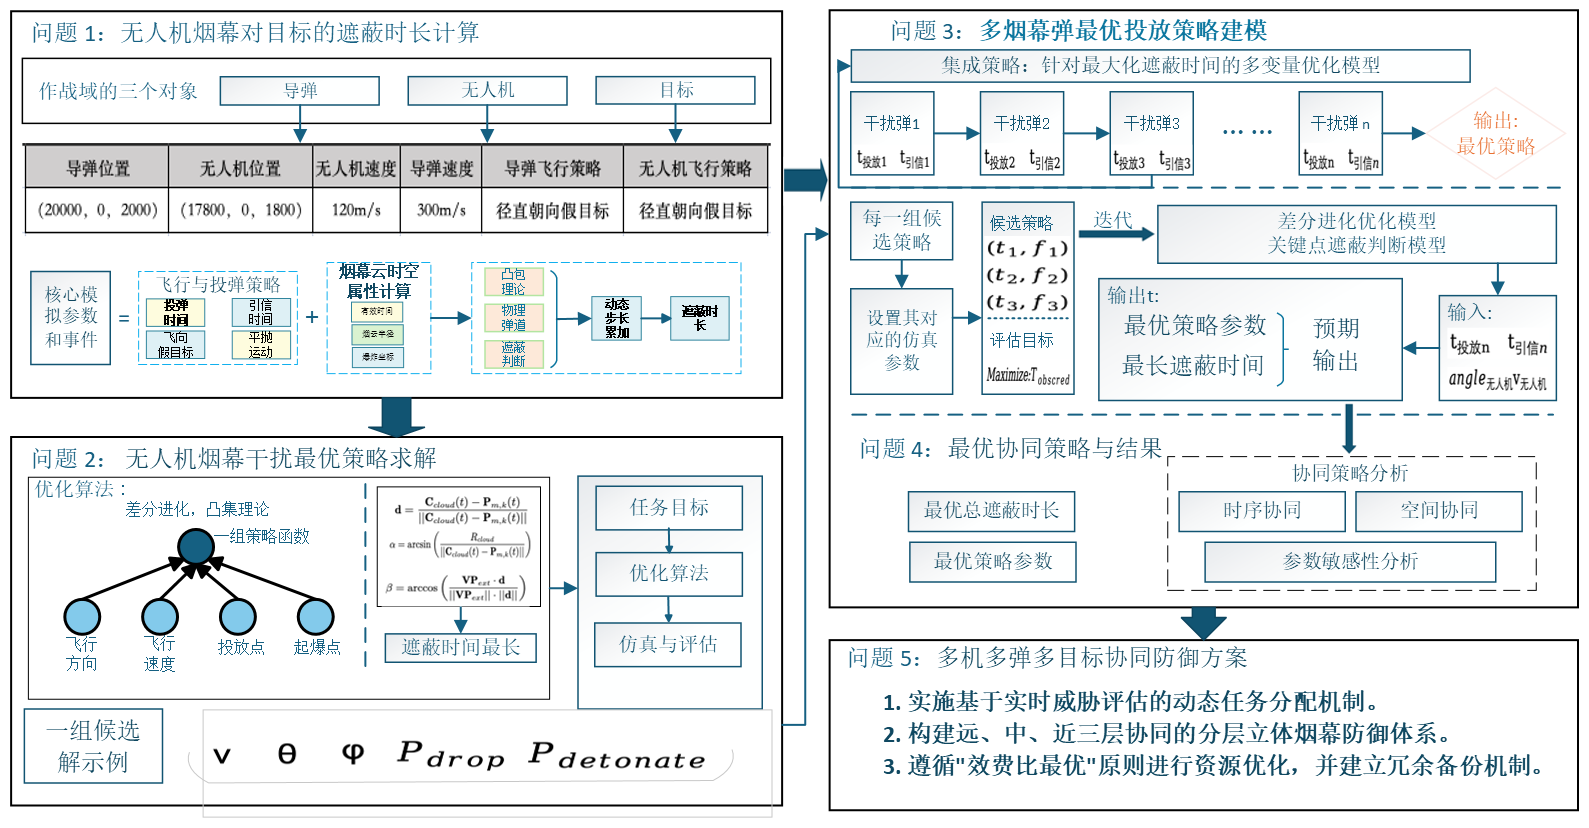
\includegraphics[width=\textwidth]{9.全文流程图.png}
    \caption{本文建模思路示意图}
    \label{fig:obscuration_cases}
\end{figure}

% ================================================= 模型、符号 =====================================================
\section{模型假设}

\begin{enumerate}[leftmargin=1cm]
    \item \textbf{平面地球假设:} 将地面视为理想的平坦平面,忽略地球的曲率与自转效应,并在此基础上建立三维笛卡尔坐标系。
    \item \textbf{理想大气假设:} 大气环境静止且均匀,无风、无湍流,空气密度等参数恒定,不随高度变化。
    \item \textbf{瞬时投放假设:} 烟雾弹从无人机投放的瞬间,其初始速度向量与无人机当时的飞行速度向量完全一致。
    \item \textbf{理想烟雾假设:} 烟雾弹起爆后瞬时形成一个半径恒定、内部均匀且完全不透明的理想球形云团。任何穿过该球体的视线都将被完全遮蔽。
    \item \textbf{云团独立性假设:} 每一个烟雾云团都是独立的遮蔽体,多个云团的遮蔽范围可以重叠,但它们之间不会发生物理或化学上的相互作用。
\end{enumerate}

\section{符号说明}

\begin{table}[H]
\centering
\caption{主要符号说明}
\begin{tabularx}{0.9\textwidth}{c C c}
\toprule
\textbf{符号} & \textbf{说明} & \textbf{单位} \\
\midrule
$\mathcal{T}_{true}$ & 真实目标圆柱体 & - \\
$\mathcal{T}_{decoy}$ & 虚拟目标点(导弹飞行朝向) & - \\
$FY_i$ & 第 $i$ 架无人机 & - \\
$M_k$ & 第 $k$ 枚导弹 & - \\
$S_{ij}$ & 无人机 $FY_i$ 投放的第 $j$ 枚烟雾弹 & - \\
$m_{grenade}$ & 单枚烟雾弹的质量 & kg \\
$g$ & 重力加速度 & m/s² \\
$\mathbf{P}_{uav, i}(t)$ & 无人机 $FY_i$ 在时刻 $t$ 的位置向量 & m \\
$v_{uav, i}$ & 无人机 $FY_i$ 的飞行速度 & m/s \\
$\theta_{uav, i}$ & 无人机 $FY_i$ 的水平飞行方向角 & rad \\
$t_{deploy, ij}$ & 烟雾弹 $S_{ij}$ 的投放时刻 & s \\
$t_{fuse, ij}$ & 烟雾弹 $S_{ij}$ 的引信时长 & s \\
\bottomrule
\end{tabularx}
\end{table}
% ================================================= 弹道计算 =====================================================
\section{前期准备}

\subsection{烟雾弹运动弹道分析}

无人机投放烟雾弹后,其在空中的飞行轨迹是一个需要综合考虑重力与空气阻力的弹道问题。运动过程中,烟雾弹主要受到两个力的作用:恒定的重力 $ \mathbf{F}_g $ 和与其瞬时速度相关的空气阻力 $ \mathbf{F}_d $。

\subsubsection{受力分析与建模}

根据牛顿第二定律,烟雾弹的运动可以由以下矢量微分方程描述:
\begin{equation}
m_{grenade} \frac{d\mathbf{v}(t)}{dt} = \mathbf{F}_g + \mathbf{F}_d
\label{eq:newton_law}
\end{equation}
其中,$m_{grenade}$ 是烟雾弹的质量,$\mathbf{v}(t)$ 是其瞬时速度向量。

\paragraph{重力建模}
重力是一个方向竖直向下、大小恒定的力。在我们的坐标系中,重力向量表示为:
\begin{equation}
\mathbf{F}_g = m_{grenade}\mathbf{g} = (0, 0, -m_{grenade}g)
\label{eq:gravity}
\end{equation}

\paragraph{空气阻力建模}
对于烟雾弹这类在空气中高速运动的物体,其所受空气阻力可以用二次阻力模型来衡量,即阻力的大小与速度的平方成正比,方向与速度方向相反。其矢量表达式为:
\begin{equation}
\mathbf{F}_d = - \frac{1}{2} C_d \rho A |\mathbf{v}(t)| \mathbf{v}(t)
\label{eq:drag_quadratic}
\end{equation}
其中,$C_d$ 是阻力系数,$\rho$ 是空气密度,$A$ 是物体的有效横截面积。为简化表达,我们将这些参数合并为一个综合性的阻力因子 $k' = \frac{1}{2} C_d \rho A$,则上式可写为:
\begin{equation}
\mathbf{F}_d = -k' |\mathbf{v}(t)| \mathbf{v}(t)
\label{eq:drag_factor}
\end{equation}

\subsubsection{运动方程的求解}

将式(\ref{eq:gravity})和式(\ref{eq:drag_factor})代入式(\ref{eq:newton_law}),我们得到烟雾弹的非线性矢量运动方程:
\begin{equation}
m_{grenade} \frac{d\mathbf{v}(t)}{dt} = m_{grenade}\mathbf{g} - k' |\mathbf{v}(t)| \mathbf{v}(t)
\label{eq:motion_vector_nonlinear}
\end{equation}

对于这个复杂的非线性常微分方程组,我们难以求得其解析解,于是,我们采用数值方法进行高精度求解。首先,把这个二阶系统转化为一个一阶系统。定义一个六维的状态向量 $\mathbf{y}(t)$:
\begin{equation}
\mathbf{y}(t) = \begin{bmatrix} \mathbf{p}(t) \\ \mathbf{v}(t) \end{bmatrix} = [x, y, z, v_x, v_y, v_z]^T
\end{equation}
其中 $\mathbf{p}(t)$ 是位置向量,$\mathbf{v}(t)$ 是速度向量。

状态向量的一阶导数为:
\begin{equation}
\frac{d\mathbf{y}}{dt} = \begin{bmatrix} \dot{\mathbf{p}}(t) \\ \dot{\mathbf{v}}(t) \end{bmatrix} = \begin{bmatrix} \mathbf{v}(t) \\ \mathbf{g} - \frac{k'}{m_{grenade}} |\mathbf{v}(t)| \mathbf{v}(t) \end{bmatrix} = f(t, \mathbf{y})
\label{eq:state_space_ode}
\end{equation}

我们采用常微分方程求解器,结合高精度的\textbf{龙格-库塔(RK45)算法}进行求解。这是一种自适应步长的算法,在保证精度的同时,也能够高效地计算出弹道轨迹。通过给定投放瞬间的初始状态(初始位置 $\mathbf{p}_0$ 和初始速度 $\mathbf{v}_0$),并求解上述常微分方程组,我们便可以精确地确定烟霏弹在预定引信时间 $t_{fuse}$ 后的准确起爆位置 $\mathbf{P}_{detonate}$。

在参考了相关空气动力学研究\cite{ref_drag_coeff}与军队技术手册\cite{ref_ammo_data}中关于炮弹物体的阻力系数与烟雾弹型号参数得出本模型中涉及的关键物理参数,取值如下表所示:

\begin{table}[H]
\centering
\caption{烟雾弹弹道模型主要参数}
\begin{tabularx}{0.9\textwidth}{c C c c}
\toprule
\textbf{参数} & \textbf{符号} & \textbf{数值} & \textbf{单位} \\
\midrule
烟雾弹质量 & $m_{grenade}$ & 5.0 & kg \\
重力加速度 & $g$ & 9.8 & m/s² \\
综合阻力因子 & $k'$ & 0.005 & kg/m \\
\bottomrule
\end{tabularx}
\label{tab:grenade_params}
\end{table}
% ================================================= 凸包遮蔽 =====================================================
\subsection{基于凸包理论的遮蔽有效性判断}

为了判断在任意时刻 $t$,烟雾云团是否能够在面对来袭导弹 $M_k$ 时成功遮蔽真实目标 $\mathcal{T}_{true}$,我们建立了以下解析几何模型——该模型的核心思想是将复杂的三维遮蔽问题,通过三次几何抽象和逻辑降维,最终转化为一个简单的角度比较问题。

\begin{figure}[H]
    \centering
    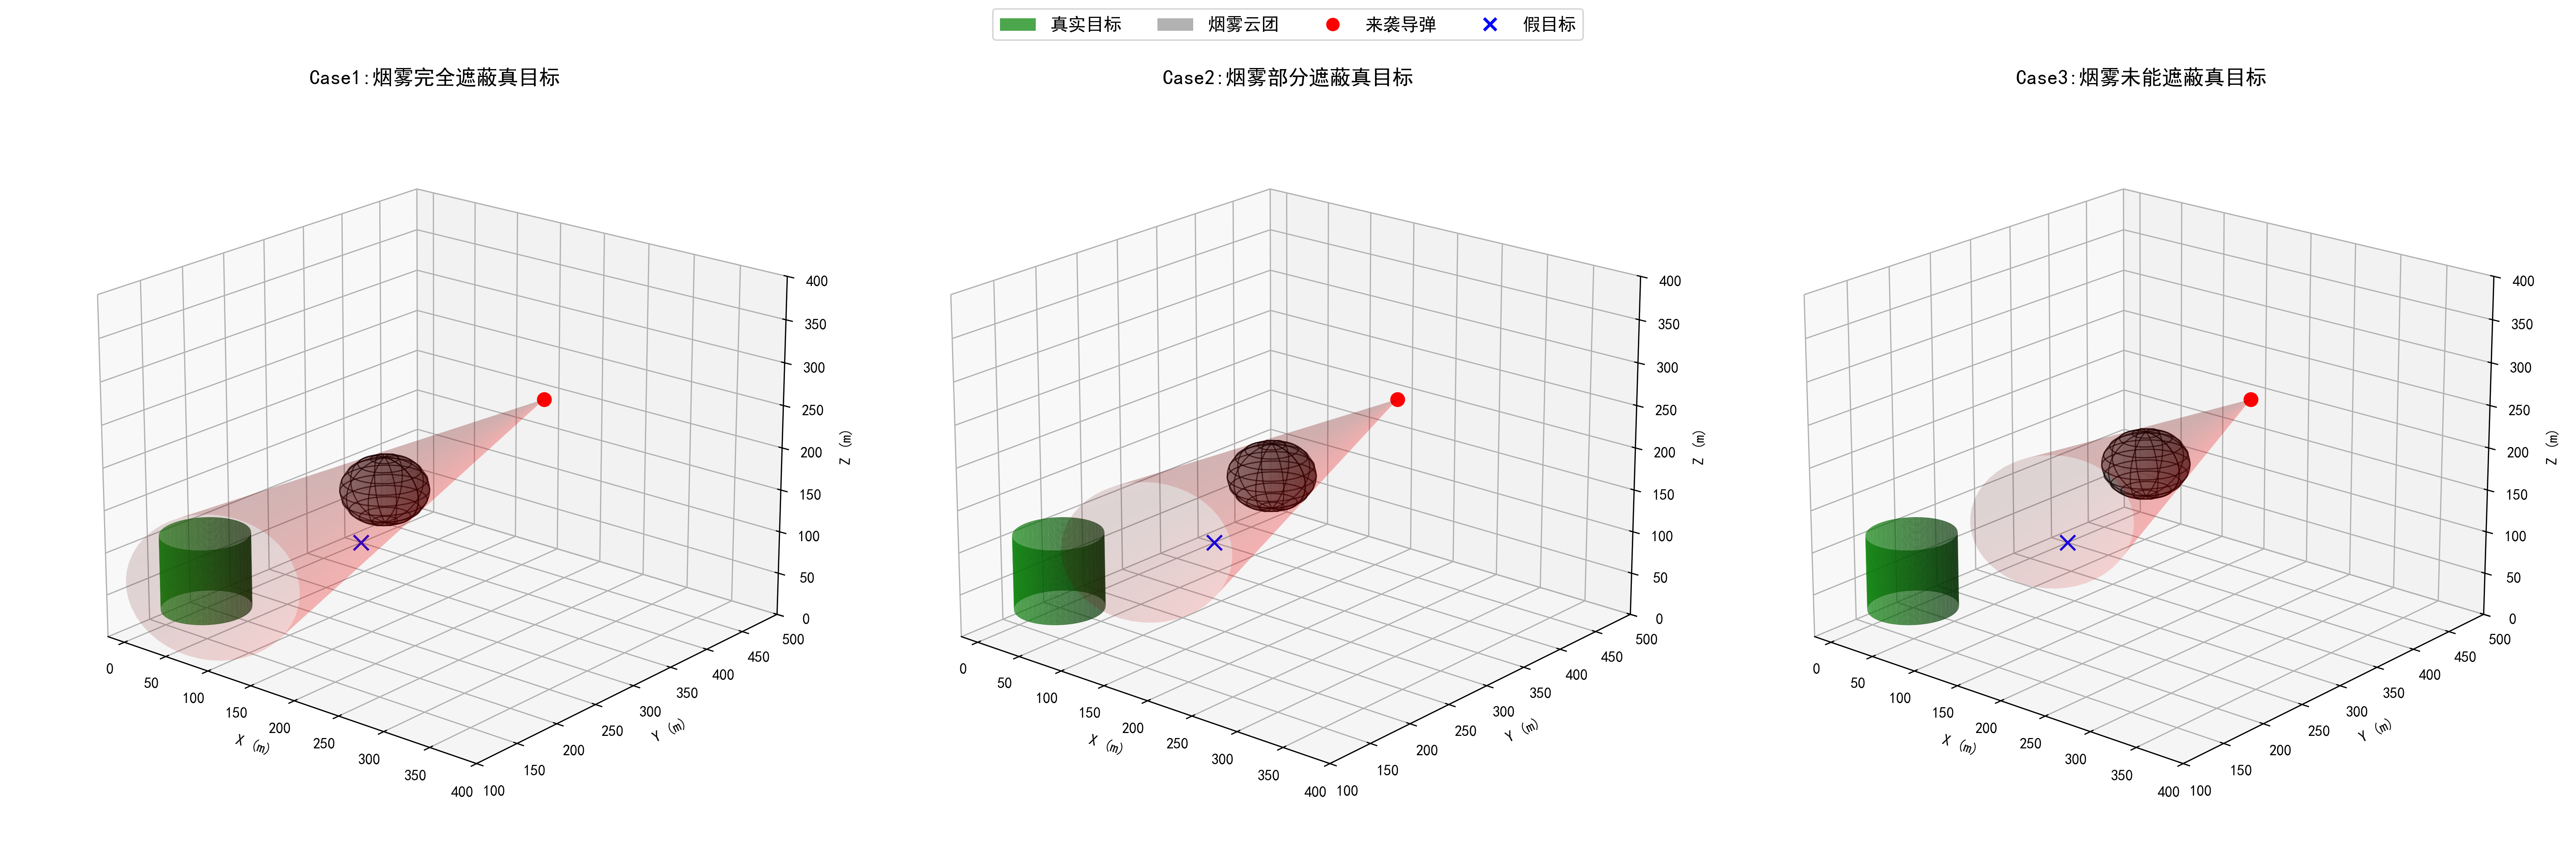
\includegraphics[width=\textwidth]{1.遮蔽效果对比图(三种情况).png}
    \caption{遮蔽有效性几何判断的三种典型情况示意图}
    \label{fig:obscuration_cases}
\end{figure}

\subsubsection{遮蔽问题的几何抽象}
我们对动态的遮蔽场景在任意时刻 $t$ 的瞬态进行分析,并将各个关键对象进行几何抽象,如图\ref{fig:obscuration_cases}所示:
\begin{itemize}
    \item \textbf{观察点 V}:将来袭导弹的瞬时位置 $\mathbf{P}_{m,k}(t)$ 抽象为一个点。
    \item \textbf{遮蔽球 S}:将烟雾云团抽象为一个半径为 $R_{cloud}$ 的理想球体,其球心为 $\mathbf{C}_{cloud}(t)$。
    \item \textbf{目标体 C}:将真实目标抽象为一个底面半径为 $r_{target}$、高为 $h_{target}$ 的标准圆柱体。
\end{itemize}

\subsubsection{基于阴影锥的判断模型}
在上述基础上,遮蔽问题可以转化为一个几何包含问题:判断目标圆柱体 C 是否完全位于观察点 V 与遮蔽球 S 所形成的“阴影锥”内部。该阴影锥的几何参数定义如下:
\begin{itemize}
    \item \textbf{锥顶点}:即观察点 V。
    \item \textbf{锥轴线单位向量 $\mathbf{d}$}:由观察点 V 指向遮蔽球球心 $\mathbf{C}_{cloud}$ 的单位向量。
    \begin{equation}
    \mathbf{d} = \frac{\mathbf{C}_{cloud}(t) - \mathbf{P}_{m,k}(t)}{||\mathbf{C}_{cloud}(t) - \mathbf{P}_{m,k}(t)||}
    \end{equation}
    \item \textbf{锥半顶角 $\alpha$}:由 V、$\mathbf{C}_{cloud}$ 和球体的大圆切线构成的直角三角形可得:
    \begin{equation}
    \alpha = \arcsin\left(\frac{R_{cloud}}{||\mathbf{C}_{cloud}(t) - \mathbf{P}_{m,k}(t)||}\right)
    \end{equation}
\end{itemize}

\subsubsection{模型降维——从圆柱体到关键圆周}
根据凸包理论,要判断一个凸体(目标圆柱体)是否完全位于另一个凸体(阴影锥)内部,我们无需检验其内部所有点。我们只需要证明目标体的轮廓完全被包含即可。对于圆柱体而言,其最关键的轮廓就是其顶部圆周 $\Omega_{top}$ 和底部圆周 $\Omega_{bottom}$。因此,我们将三维的体包含问题,降维为两个独立的二维圆周包含问题。

\begin{figure}[H]
    \centering
    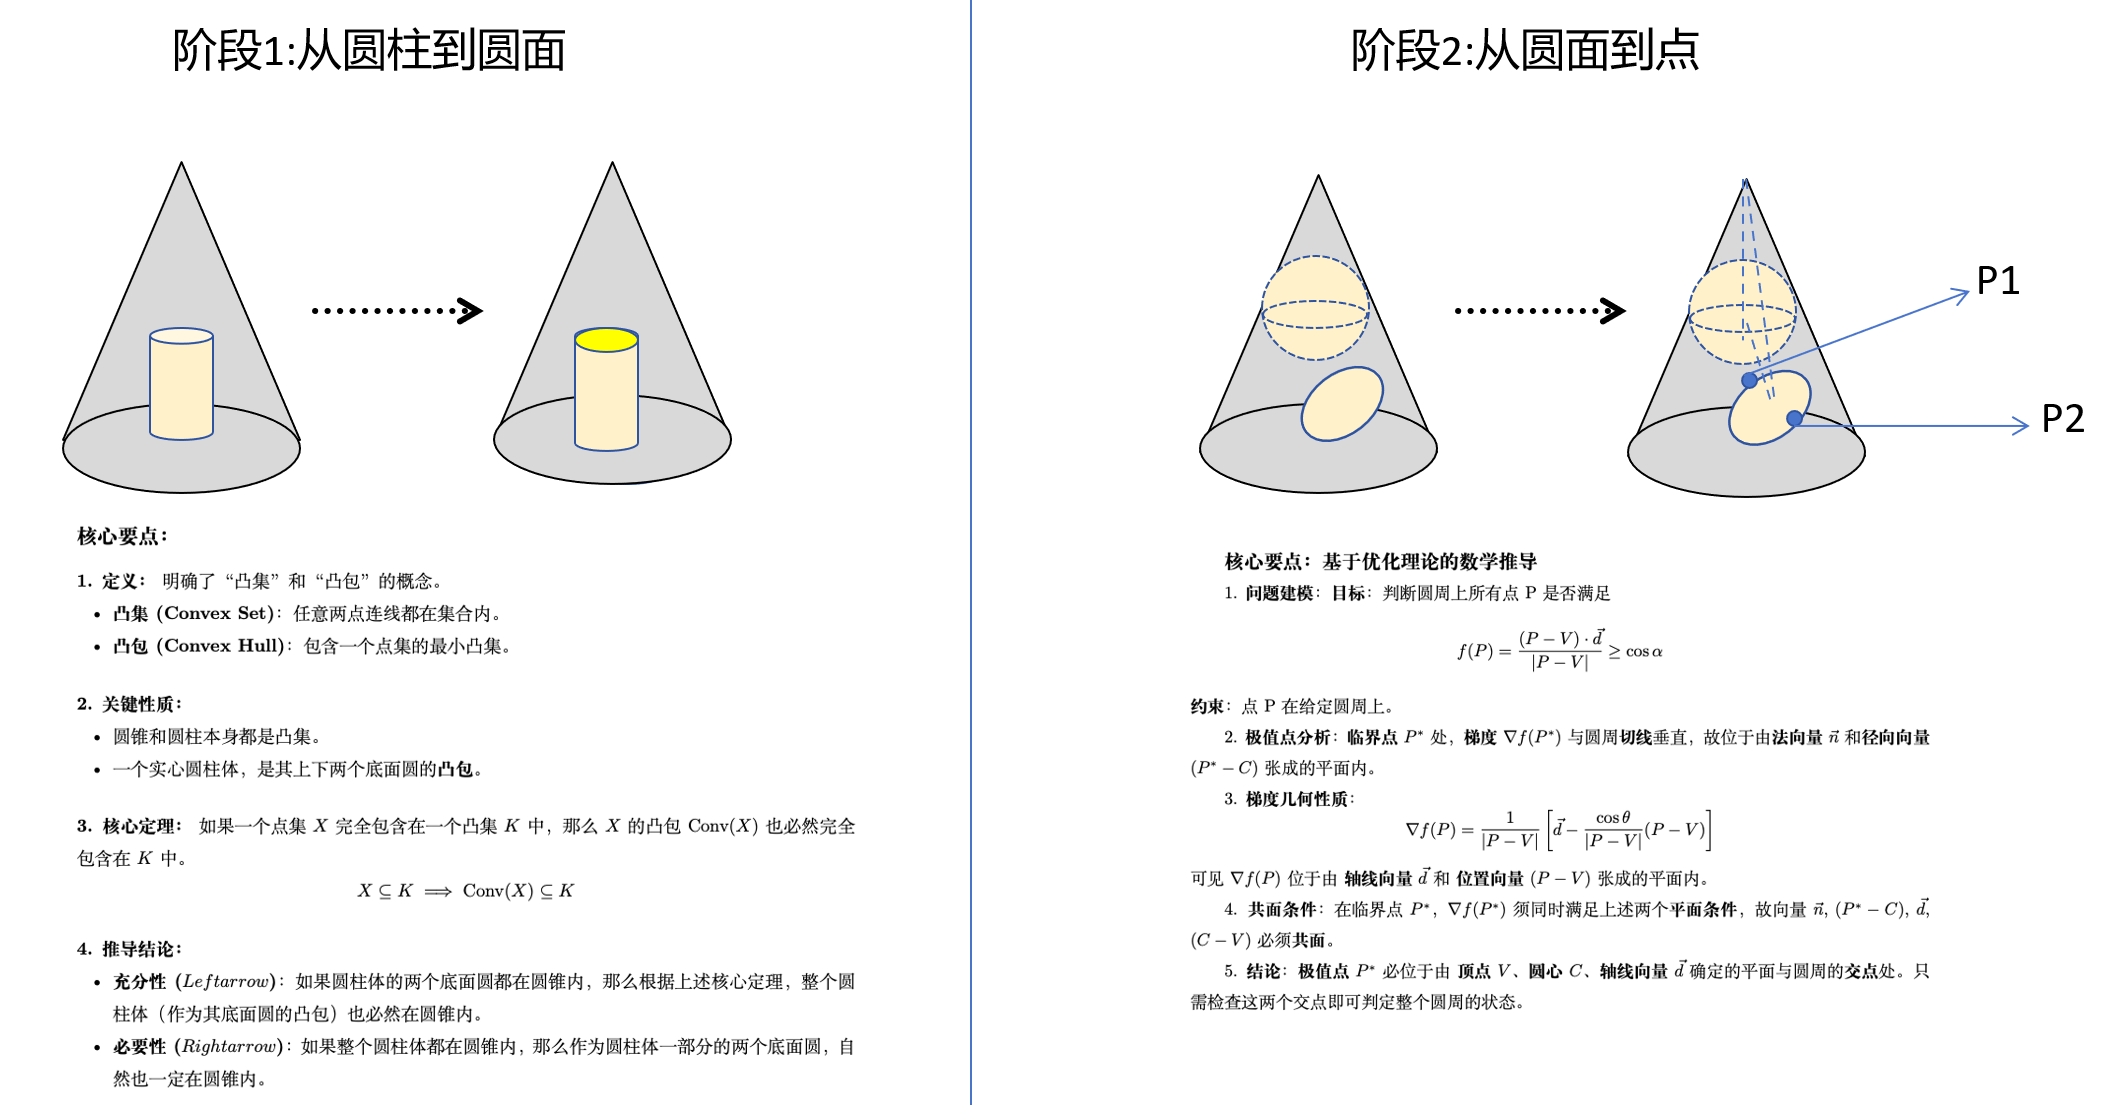
\includegraphics[width=\textwidth]{8.凸包理论阶段2-3示意图.png}
    \caption{遮蔽有效性几何判断的三种典型情况示意图}
    \label{凸包理论模型降维与圆周极值点解析示意图}
\end{figure}

\subsubsection{关键点判断——从圆周到极值点}
进一步地,要判断一个完整的圆周 $\Omega$ 是否在阴影锥内,我们同样无需遍历圆周上的所有点。我们只需要找到该圆周上最有可能溢出阴影锥的两个极值 $\mathbf{P}_{ext1}$ 和 $\mathbf{P}_{ext2}$。

这两个极值点可以通过几何方法确定:它们位于由锥顶点 V、圆周中心 $\mathbf{C}_{\Omega}$ 和锥轴线 $\mathbf{d}$ 所构成的“关键平面”与圆周平面 $\Pi_{\Omega}$ 的交线上。

对于任意一个极值点 $\mathbf{P}_{ext}$,我们计算其与锥顶点V的连线向量 $\mathbf{V}\mathbf{P}_{ext}$ 和锥轴线向量 $\mathbf{d}$ 之间的夹角,即检验角 $\beta$:
\begin{equation}
\beta = \arccos\left( \frac{\mathbf{V}\mathbf{P}_{ext} \cdot \mathbf{d}}{||\mathbf{V}\mathbf{P}_{ext}|| \cdot ||\mathbf{d}||} \right)
\end{equation}

如果目标圆柱体顶部和底部两个圆周的所有极值点所对应的检验角 $\beta$ 均满足 $\beta \le \alpha$,则我们判定目标在该时刻被完全遮蔽。

\subsubsection{核心判断逻辑伪代码}
整个判断流程的核心逻辑可以由以下伪代码概括:

\begin{algorithm}[H]
\caption{遮蔽有效性判断核心算法}
\begin{algorithmic}[1]
\STATE \textbf{Function} IsObscured($\mathbf{P}_{missile}$, $\mathbf{C}_{cloud}$, $\mathcal{T}_{target}$)
\STATE   构建阴影锥 (顶点 $\mathbf{V} \leftarrow \mathbf{P}_{missile}$, 轴线 $\mathbf{d}$, 半顶角 $\alpha$)
\STATE   获取目标圆柱体的顶部圆周 $\Omega_{top}$ 和底部圆周 $\Omega_{bottom}$
\STATE   \textbf{For Each} 圆周 $\Omega$ in $\{\Omega_{top}, \Omega_{bottom}\}$:
\STATE     \quad 确定该圆周的两个极值点 $\mathbf{P}_{ext1}, \mathbf{P}_{ext2}$
\STATE     \quad \textbf{For Each} 极值点 $\mathbf{P}_{ext}$ in $\{\mathbf{P}_{ext1}, \mathbf{P}_{ext2}\}$:
\STATE     \qquad   计算检验角 $\beta \leftarrow \text{AngleBetween}(\vec{\mathbf{V}\mathbf{P}_{ext}}, \mathbf{d})$
\STATE     \qquad   \textbf{If} $\beta > \alpha$:
\STATE     \qquad     \quad \textbf{Return} False  \COMMENT{遮蔽无效}
\STATE   \textbf{Return} True  \COMMENT{遮蔽有效}
\end{algorithmic}
\end{algorithm}
% ================================================= 建模求解 =====================================================
\section{模型的建立与求解}
% ================================================= 题一求解 =====================================================
\subsection{问题一的模型建立与求解}

\begin{figure}[H]
    \centering
    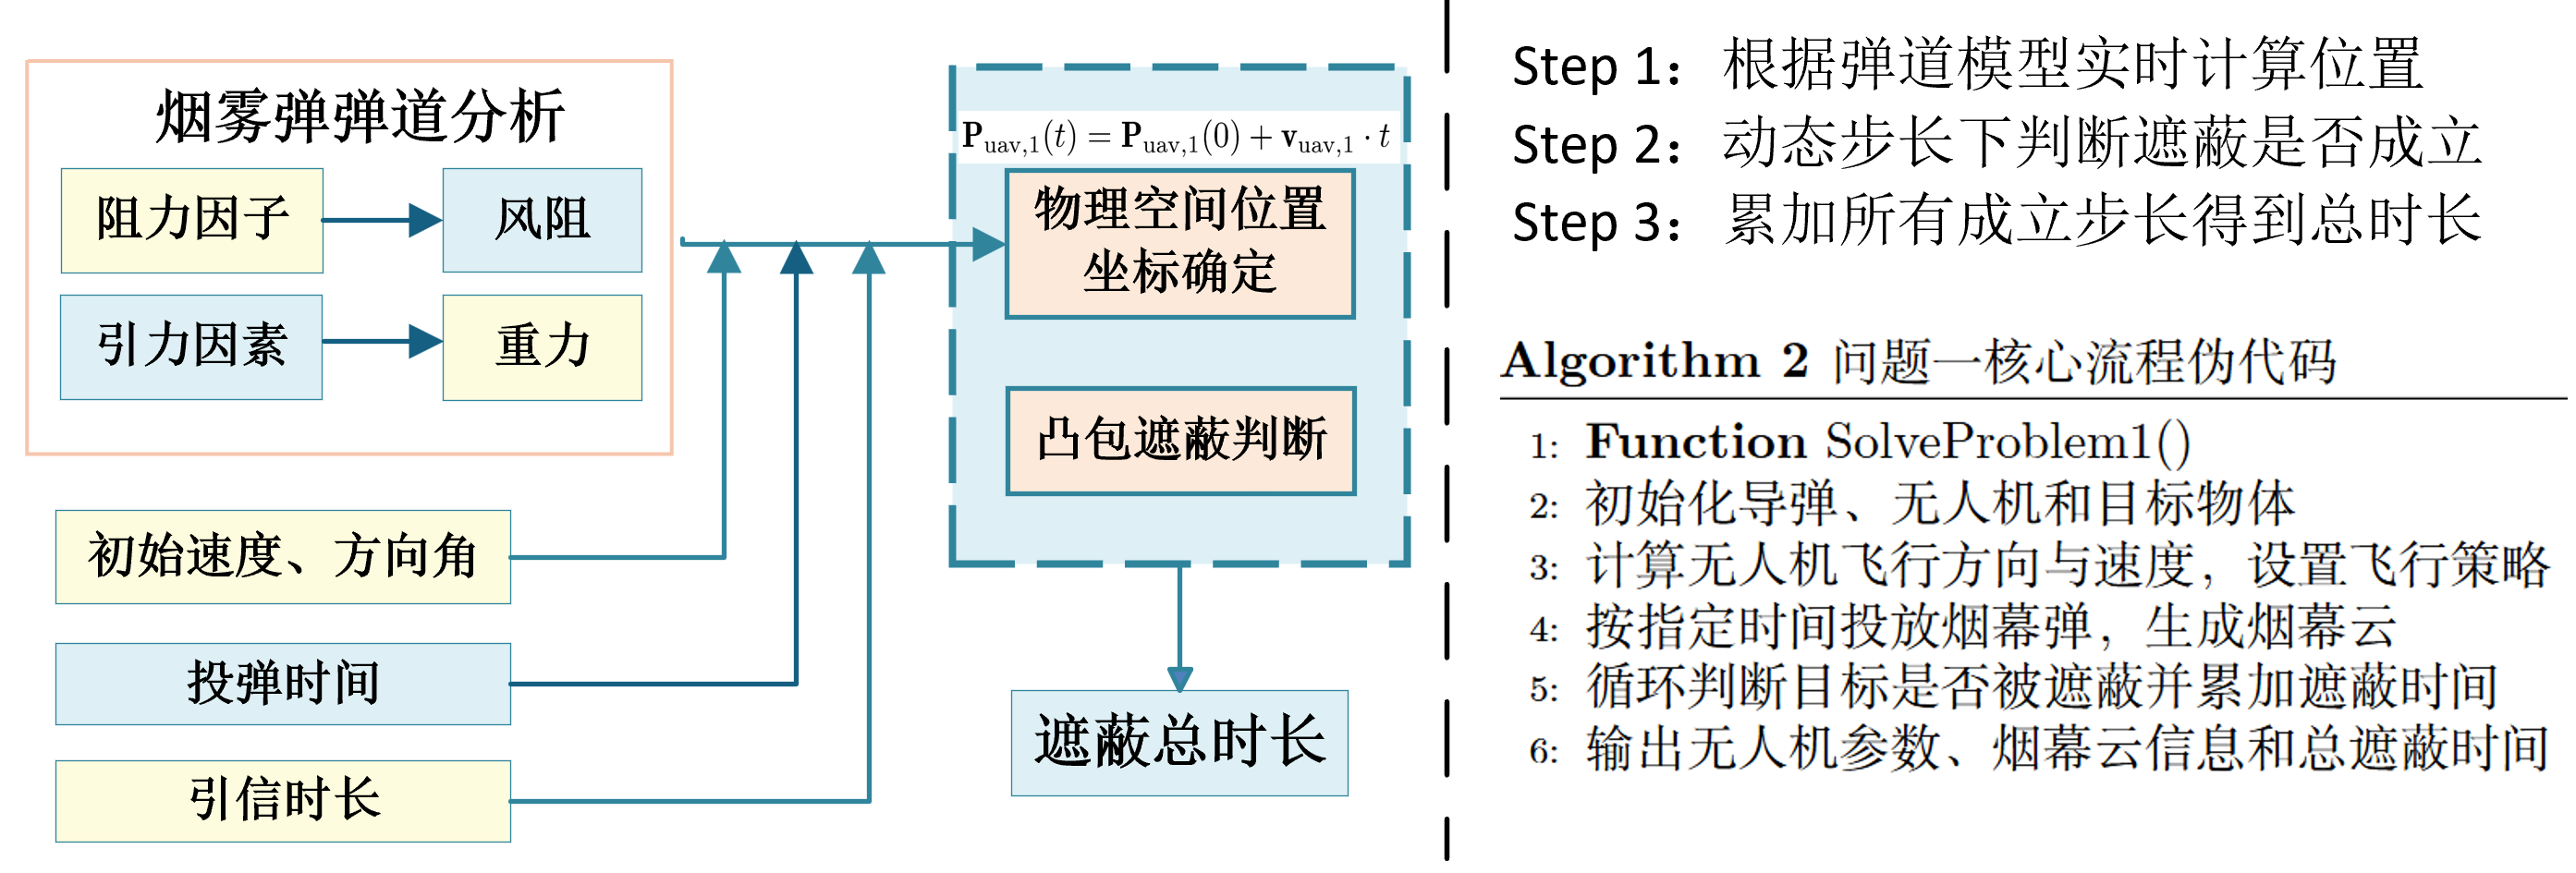
\includegraphics[width=0.86\textwidth]{7.问题1流程图.png}
    \caption{问题一整体流程示意图}
    \label{fig:obscuration_cases}
\end{figure}


\subsubsection{无人机匀速直线飞行求解}
对于问题一,无人机FY1以$v_{\text{uav},1} = 120 \, \text{m/s}$的恒定速率,朝向假目标$\mathcal{T}_{\text{decoy}}$飞行。这是一个标准的匀速直线运动模型,无人机在任意时刻$t$的位置$\mathbf{P}_{\text{uav},1}(t)$可通过下式计算:
\begin{equation}
    \mathbf{P}_{\text{uav},1}(t) = \mathbf{P}_{\text{uav},1}(0) + \mathbf{v}_{\text{uav},1} \cdot t
\end{equation}

其中,$\mathbf{P}_{\text{uav},1}(0)$为无人机初始位置,$\mathbf{v}_{\text{uav},1}$为其速度矢量。根据题目设定,在$t_{\text{deploy},1,1} = 1.5 \, \text{s}$时,无人机执行投弹操作,此刻无人机的位置和速度,即为烟幕弹$S_{1,1}$在被投放时的初始运动状态。

\subsubsection{烟幕弹弹道模型应用}
烟幕弹$S_{1,1}$被投放后,其运动轨迹主要受重力和空气阻力的共同影响。我们在5.1节中已经建立了完善的动力学模型。其核心状态方程组如下:
\begin{equation}
    \frac{d\mathbf{r}}{dt} = \mathbf{v}
\end{equation}
\begin{equation}
    m_{\text{grenade}}\frac{d\mathbf{v}}{dt} = m_{\text{grenade}}\mathbf{g} - \frac{1}{2} C_d \rho A \lVert\mathbf{v}\rVert \mathbf{v}
\end{equation}

我们将无人机在$1.5 \, \text{s}$时的位置和速度作为该微分方程组的初始条件,引信时长$t_{\text{fuse},1,1} = 3.6 \, \text{s}$作为积分时长。通过调用高阶的数值积分方法(如RK45),我们能够精确求解出烟幕弹在$t=1.5+3.6=5.1 \, \text{s}$时刻的爆炸点三维坐标。

\begin{figure}[htbp]
    \centering
    \makebox[\linewidth][c]{%
        % 路径已修正为直接使用文件名
        \includegraphics[width=1.2\textwidth]{{2.问题一关键时刻空中态势图.png}}
    }
    \caption{问题一中三个关键时刻的空中态势演变图}
    \label{fig:problem1_moments}
\end{figure}

\subsubsection{遮蔽判断与遮蔽时长计算}
烟幕云在$t=5.1 \, \text{s}$时于爆炸点生成,其作为一个半径为$R=10 \, \text{m}$的球体,并以$v_{\text{sink}}=3 \, \text{m/s}$的速度下沉,持续时间为$T_{\text{cloud}}=20 \, \text{s}$。在此期间,我们建立了一个离散时间的仿真程序,以$\Delta t = 0.01 \, \text{s}$为步长,从$t=5.1 \, \text{s}$到$t=25.1 \, \text{s}$进行循环检测。在每一个时间步$t_i$,我们都会动态更新导弹M1的位置$\mathbf{P}_{\text{M1}}(t_i)$和烟雾云中心的位置$\mathbf{P}_{\text{cloud}}(t_i)$,并调用5.2节建立的几何遮蔽判断模型,检验真实目标$\mathcal{T}_{\text{true}}$此时是否被完全遮蔽。若遮蔽成立,则累加该时间步长$\Delta t$。仿真结束后,累加的总时长即为问题一的解。

\textbf{经过上述仿真计算,最终得到烟幕干扰弹对M1的有效遮蔽总时长为:$\mathbf{1.3200 \, s}$。}
% ================================================= 题二求解 =====================================================
\subsection{问题二的模型建立与求解}

在问题一的物理基础上,问题二将原本固定的飞行策略转变为可优化的决策,构建了一个四维连续优化问题。我们采用差分进化算法作为全局优化求解器,综合考虑无人机飞行动力学、烟雾弹弹道和三维几何遮蔽判断,在复杂的目标函数空间中寻找最优解。

\begin{figure}[H]
    \centering
    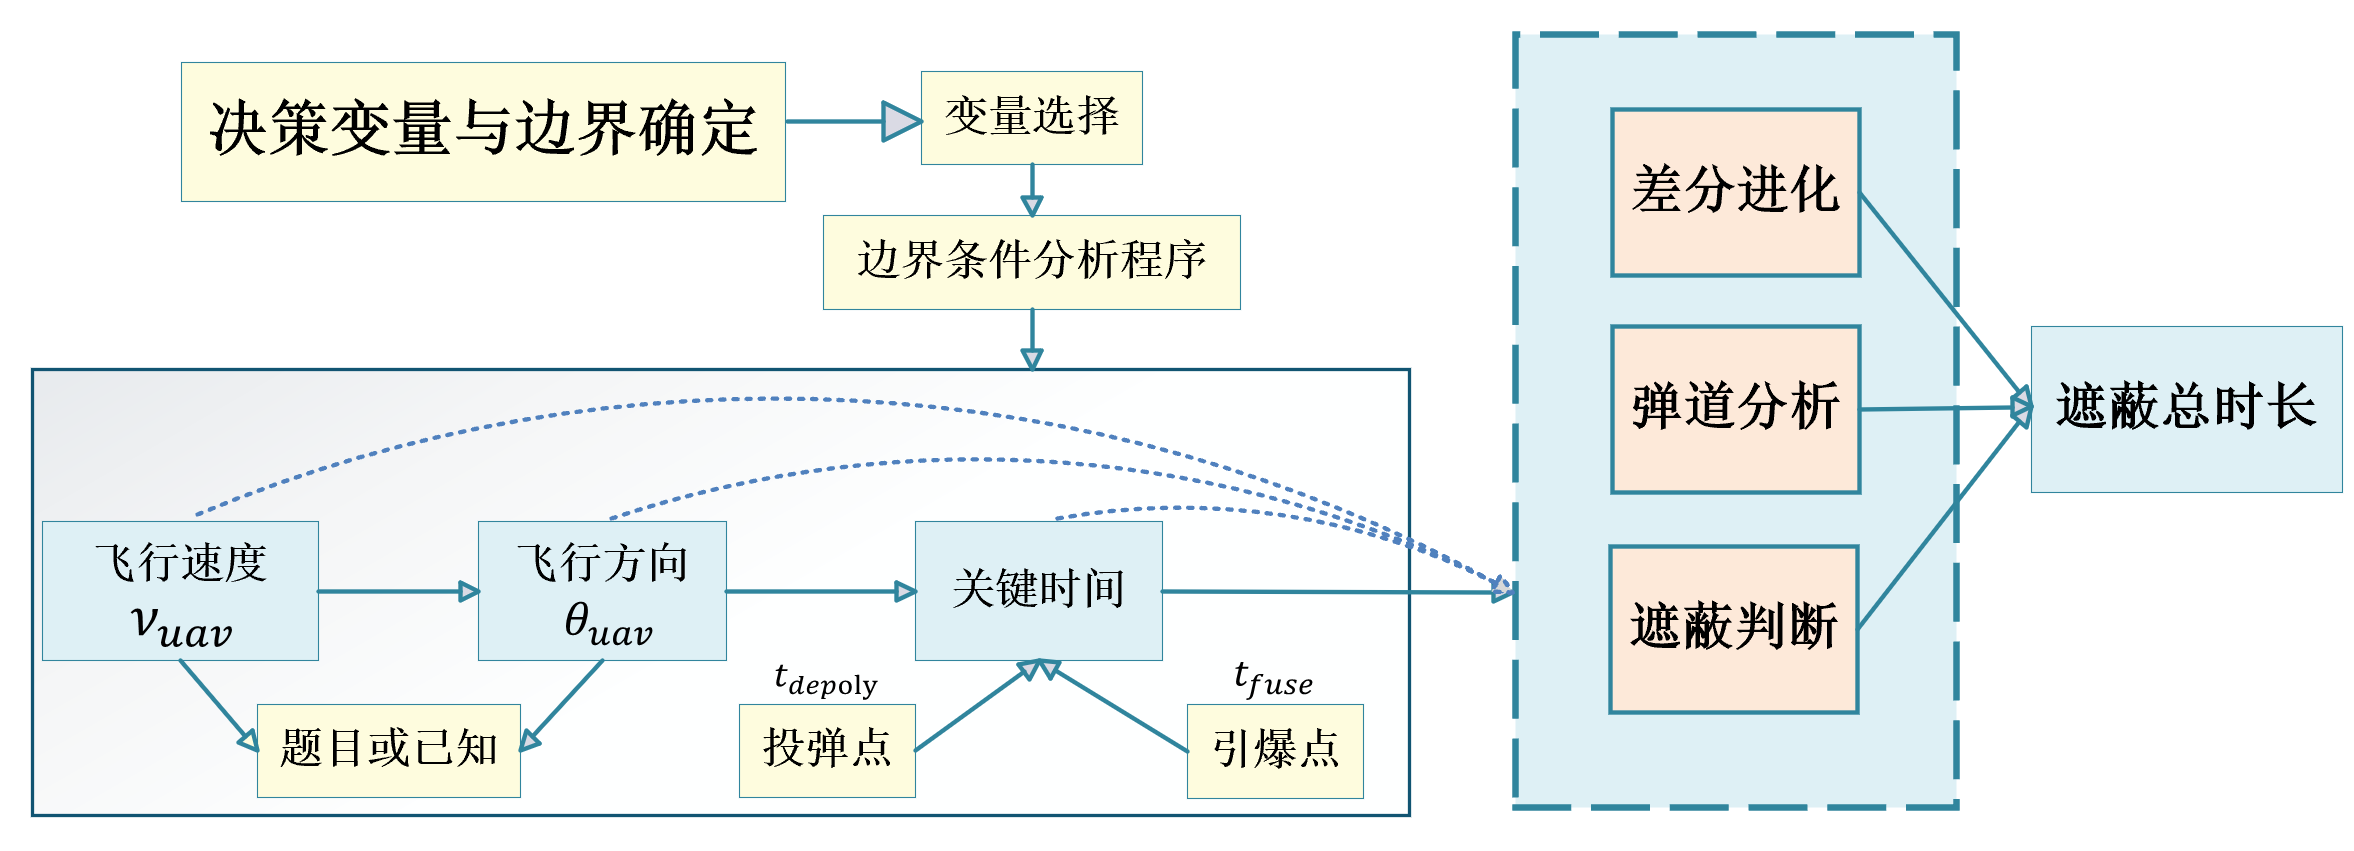
\includegraphics[width=0.84\textwidth]{5.问题2流程图.png}
    \caption{问题二整体流程示意图}
    \label{fig:obscuration_cases}
\end{figure}

\subsubsection{决策变量选择与边界条件确定}

问题二的决策变量包括四个维度,各变量及其边界条件如表\ref{tab:problem2_variables}所示。

\begin{table}[H]
\centering
\caption{问题二决策变量及边界条件}
\begin{tabularx}{0.9\textwidth}{c C c c}
\toprule
\textbf{决策变量} & \textbf{符号} & \textbf{边界条件} & \textbf{单位} \\
\midrule
无人机飞行速度 & $v_{uav}$ & [70, 140] & m/s \\
无人机飞行方向角 & $\theta$ & [0, 2$\pi$] & rad \\
烟雾弹投放时间 & $t_{deploy}$ & [0.1, 13.9] & s \\
烟雾弹引信时长 & $t_{fuse}$ & [0.1, 26.7] & s \\
\bottomrule
\end{tabularx}
\label{tab:problem2_variables}
\end{table}

无人机飞行速度边界由题目明确规定,反映了无人机的物理性能约束。飞行方向角采用全方向搜索策略,允许算法自主发现最优飞行方向。

\textbf{对于时间相关的决策变量,我们使用专门的边界分析程序确定合理范围:}
通过几何约束分析确定\textbf{烟雾弹投放时间}的上界,采用极端策略(最大飞行速度、最优飞行方向、极值引信时间)进行边界扫描,确保烟雾云能够在空间上位于导弹与真目标之间,避免无效的搜索空间。\textbf{引信时长}的上界基于烟雾弹从1800米高度的物理落地时间计算,结合5.1节中建立的烟雾弹弹道模型,计算得出烟雾弹的最大飞行时间约为26.6秒,若引信时长超过此值,烟雾弹将在起爆前落地,失去遮蔽意义。

\subsubsection{差分进化优化模型建立}

在上述基础上,我们构建了基于差分进化算法的全局优化模型,其核心架构包括目标函数设计和进化算法实现两个部分。

目标函数采用离散时间仿真方法计算有效遮蔽总时长。给定决策变量向量后,首先调用问题一中建立的烟雾弹弹道计算模型和几何遮蔽判断模型,然后在烟雾云有效持续时间内以0.1秒为步长进行时间离散化,逐步检查每个时刻的遮蔽状态,最终累加得到总遮蔽时间作为优化目标。

差分进化算法是一种基于种群的随机搜索方法,适合处理本题这种非线性、多模态的连续优化问题。算法通过变异、交叉和选择三个操作实现种群进化:变异操作利用种群中个体间的差分向量产生候选解,交叉操作结合当前个体与候选解的信息,选择操作则是保留适应度更高的个体。我们设置种群规模为300(75倍问题维度),最大迭代次数6000次,而且启用并行计算提高了求解效率。

\subsubsection{模型求解结果}

\textbf{求解得到问题二的最优策略,最大有效遮蔽时间为4.7000 s,最优决策变量及关键位置信息如表\ref{tab:problem2_results}所示。}

\begin{table}[H]
\centering
\caption{问题二最优求解结果}
\begin{tabularx}{\textwidth}{c C c}
\toprule
\textbf{参数类型} & \textbf{参数名称} & \textbf{最优值} \\
\midrule
\multirow{5}{*}{最优决策变量} & 无人机FY1飞行速度 & 79.6123 m/s \\
 & 无人机FY1飞行方向 & 0.1271 rad (7.28°) \\
 & 烟雾弹投放时间 & 0.2306 s \\
 & 烟雾弹引信时长 & 0.5782 s \\
 & 烟雾弹起爆时间 & 0.8088 s \\
\midrule
\multirow{3}{*}{关键位置信息} & 投放点坐标 & (17818.21, 2.33, 1800.00) m \\
 & 起爆点坐标 & (17862.85, 8.03, 1798.39) m \\
 & 导弹M1在起爆时刻位置 & (19758.58, 0.00, 1975.86) m \\
\bottomrule
\end{tabularx}
\label{tab:problem2_results}
\end{table}

优化结果表明,相比问题一的固定策略(遮蔽时间1.3200 s),通过参数优化将遮蔽效果提升至4.7000 s,遮蔽时间增加了3.56倍。值得指出的是,由于步长选择问题,计算得到的最优参数有几组接近的不同解,尽管最终的遮蔽时间均为4.7000 s,我们这里只放出一组示范。
% ================================================= 题三求解 =====================================================
\subsection{问题三的模型建立与求解}

\subsubsection{凸包理论遮蔽判断的局限性与关键点遮蔽判断的提出}

\begin{figure}[H]
    \centering
    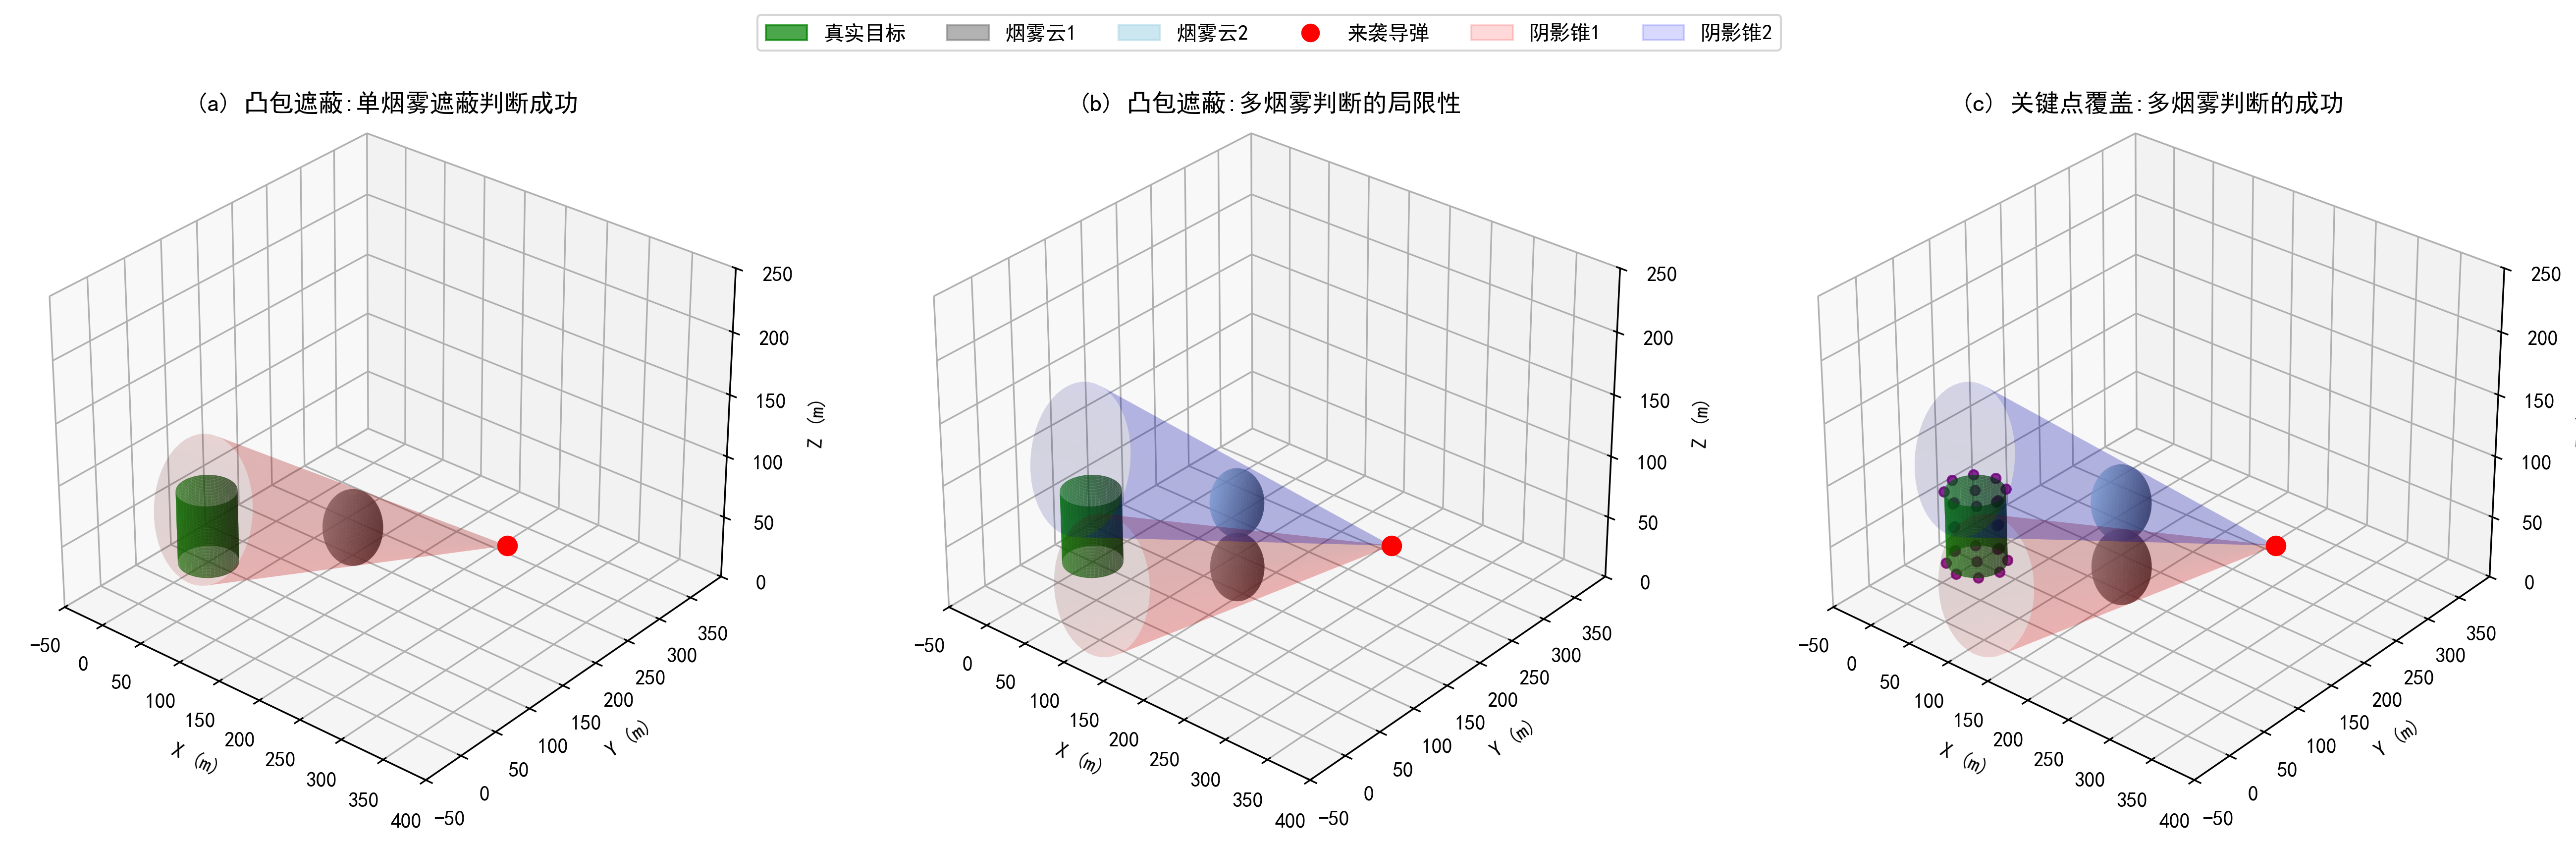
\includegraphics[width=\textwidth]{3.凸集局限与关键点覆盖对比图.png}
    \caption{凸包局限性与关键点覆盖法示意图}
    \label{fig:obscuration_cases}
\end{figure}

在问题一、二的单烟雾场景,如图\ref{fig:obscuration_cases}(a)所示,我们采用的基于凸包理论的遮蔽判断方法十分有效:通过检查圆柱体顶部和底部圆周的极值点是否完全位于单个阴影锥内,来判断整个目标是否被遮蔽。\textbf{但是随着问题三引入多枚烟雾弹时,这种方法有所局限:当单个烟雾云只能遮蔽目标的部分区域,凸包理论方法会判定遮蔽失败,如图\ref{fig:obscuration_cases}(b),即使多个烟雾云协同工作实际上已经完全覆盖了目标。}

为解决这一问题,我们提出了基于关键点覆盖的多烟雾协同遮蔽判断方法,如图\ref{fig:obscuration_cases}(c):将圆柱体目标表面离散化为有限个关键点集,如果每个关键点至少被一个烟雾云的阴影锥覆盖,则判断协同遮蔽的有效性。\textbf{该方法实现了从"单一完全包含"到"群体协同覆盖"的转化,符合多烟雾场景的物理实际。}

\subsubsection{关键点覆盖协同遮蔽判断算法}

针对多烟雾协同遮蔽的判断需求,设计基于关键点覆盖的几何算法,包含如下两个主要的步骤:目标表面关键点生成与多阴影锥协同覆盖判断。

\textbf{关键点生成策略:}将圆柱体目标表面离散化为有限关键点集$\mathcal{P} = \{p_1, p_2, \ldots, p_N\}$,采用分层采样策略:
\begin{equation}
\mathcal{P} = \mathcal{P}_{bottom} \cup \mathcal{P}_{top} \cup \mathcal{P}_{side}
\end{equation}

其中上下底面圆周点$\mathcal{P}_{bottom/top}$通过角度均匀分割生成:
\begin{equation}
p_{i,j} = C_{bottom/top} + r_{target} \cdot [\cos(\frac{2\pi i}{n_{circ}}), \sin(\frac{2\pi i}{n_{circ}}), 0]^T
\end{equation}

侧面$\mathcal{P}_{side}$按照高度进行分层采样,确保覆盖圆柱体完整外表面。

\textbf{协同遮蔽判断算法:}给定导弹位置$\mathbf{m}$和活跃烟雾云中心集合$\{\mathbf{c}_1, \mathbf{c}_2, \ldots, \mathbf{c}_k\}$,构建对应的阴影锥集合。对每个烟雾云$i$,其阴影锥的轴向量和半角分别为:
\begin{equation}
\mathbf{d}_i = \frac{\mathbf{c}_i - \mathbf{m}}{|\mathbf{c}_i - \mathbf{m}|}, \quad \alpha_i = \arcsin\left(\frac{R_{cloud}}{|\mathbf{c}_i - \mathbf{m}|}\right)
\end{equation}

协同遮蔽成立的充要条件为:
\begin{equation}
\forall p_j \in \mathcal{P}, \exists i \in \{1,2,\ldots,k\}: \arccos\left(\frac{(\mathbf{p}_j - \mathbf{m}) \cdot \mathbf{d}_i}{|\mathbf{p}_j - \mathbf{m}|}\right) \leq \alpha_i
\end{equation}

\subsubsection{多弹时序差分进化优化模型}

\textbf{边界条件分析与沿用:}
问题三的决策变量扩展为8维向量$\mathbf{x} = [v, \theta, t_{d1}, t_{f1}, \Delta t_2, t_{f2}, \Delta t_3, t_{f3}]^T$。由于无人机FY1与导弹M1等关键对象没有改变,仅是增加了投弹数量,容易证明第三题中,其边界条件会更加严格,因此我们沿用问题二的边界条件即可确保最优解一定落在其中。

\textbf{时序参数化策略:}采用"基准时间+增量时间"的参数化方式避免弹药投放冲突:
\begin{equation}
\begin{cases}
t_{deploy,1} = t_{d1} \\
t_{deploy,2} = t_{d1} + \Delta t_2 \\
t_{deploy,3} = t_{d1} + \Delta t_2 + \Delta t_3
\end{cases}
\end{equation}

其中$\Delta t_2, \Delta t_3 \geq 1.0$s确保投放间隔的物理合理性。

\textbf{优化目标函数:}在离散时间网格上计算总遮蔽时间:
\begin{equation}
f(\mathbf{x}) = \max \sum_{t \in T_{grid}} \mathbb{I}[\text{协同遮蔽}(t)] \cdot \Delta t
\end{equation}

其中$\mathbb{I}[\cdot]$为示性函数,通过关键点覆盖算法判断时刻$t$的协同遮蔽状态。针对8维度优化问题,根据15倍种群规模对应1个维度的原则,我们设置差分进化算法的种群规模设置为150,最大迭代数1000,并启用并行计算加速收敛。

\subsubsection{模型求解结果与分析}

\begin{figure}[H]
    \centering
    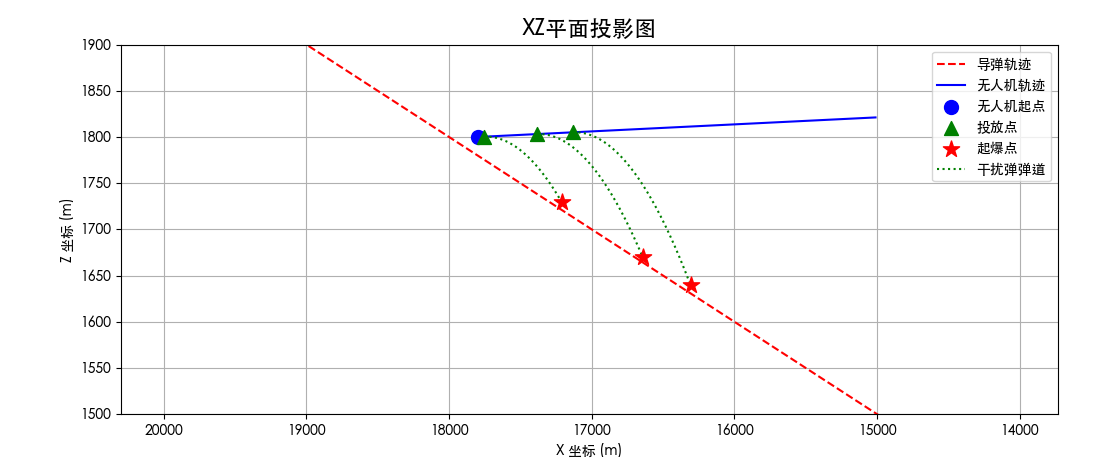
\includegraphics[width=\textwidth]{6.问题3中烟雾弹投掷zx方向视图.png}
    \caption{三枚烟雾投出后各物体位置示意图-沿zx方向}
    \label{fig:obscuration_cases}
\end{figure}

\textbf{求解得到问题三的最优协同策略如下表\ref{tab:problem3_results}所示,得到最长遮蔽时间为6.800 s。}不难看出,三弹协同策略将遮蔽时间从第二问的单弹最优4.7s提升至6.8s,性能增益44.7\%,同时采用时间梯度分布投放(间隔2.66s和1.81s),引信时间递增设计确保烟雾云接力覆盖。有意思的是,此时无人机以近最大速度(139.44 m/s)近乎沿着 -x轴方向飞行(179.53°),与第一问方向几乎相同,但是题三中飞机出发后很快投出第一枚烟雾弹,这应该是相比第一问在遮蔽时长上有巨大提升的重要原因。最终相关结果保存至result1.xlsx文件中。

\begin{table}[H]
\centering
\caption{问题三最优求解结果}
\begin{tabularx}{\textwidth}{c C c}
\toprule
\textbf{参数类型} & \textbf{参数名称} & \textbf{最优值} \\
\midrule
\multirow{2}{*}{无人机策略} & 飞行速度 & 139.4411 m/s \\
 & 飞行角度 & 3.1340 rad (179.53°) \\
\midrule
\multirow{2}{*}{干扰弹1} & 投放时间 & 0.3146 s \\
 & 引信时间 & 3.8931 s \\
\midrule
\multirow{2}{*}{干扰弹2} & 投放时间 & 2.9706 s \\
 & 引信时间 & 5.3031 s \\
\midrule
\multirow{2}{*}{干扰弹3} & 投放时间 & 4.7841 s \\
 & 引信时间 & 5.9167 s \\
\bottomrule
\end{tabularx}
\label{tab:problem3_results}
\end{table}
% ================================================= 题四求解 =====================================================
\subsection{问题四的模型建立与求解}

\subsubsection{多机协同优化框架设计及边界条件设置}

问题四将决策变量扩展为12维向量:$\mathbf{x} = [v_1, \theta_1, t_{d1}, t_{f1}, v_2, \theta_2, t_{d2}, t_{f2}, v_3, \theta_3, t_{d3}, t_{f3}]^T$,其中每组4个参数分别对应FY1、FY2、FY3三架无人机的飞行速度、方向角、投放时间和引信时长。

与问题三的增量时间参数化不同、但与问题二类似,问题四采用独立的参数化策略:各无人机的投放时间完全独立,无时序约束,通过优化算法自主发现最佳空间-时间协调模式。由于三架无人机独立执行任务,参考\ref{tab:problem2_variables}中的边界条件计算方法,用边界分析程序为每架无人机确定投弹时间与引信时间的上界,得到各变量边界条件如表\ref{tab:problem4_variables}所示。

\begin{table}[H]
\centering
\caption{问题四决策变量及边界条件}
\begin{tabularx}{0.9\textwidth}{c C c c}
\toprule
\textbf{无人机} & \textbf{决策变量} & \textbf{边界条件} & \textbf{单位} \\
\midrule
\multirow{4}{*}{FY1} & 飞行速度 $v_1$ & [70, 140] & m/s \\
 & 飞行方向角 $\theta_1$ & [0, 2$\pi$] & rad \\
 & 投放时间 $t_{d1}$ & [0.1, 13.9] & s \\
 & 引信时长 $t_{f1}$ & [0.1, 26.7] & s \\
\midrule
\multirow{4}{*}{FY2} & 飞行速度 $v_2$ & [70, 140] & m/s \\
 & 飞行方向角 $\theta_2$ & [0, 2$\pi$] & rad \\
 & 投放时间 $t_{d2}$ & [0.1, 49.7] & s \\
 & 引信时长 $t_{f2}$ & [0.1, 22.5] & s \\
\midrule
\multirow{4}{*}{FY3} & 飞行速度 $v_3$ & [70, 140] & m/s \\
 & 飞行方向角 $\theta_3$ & [0, 2$\pi$] & rad \\
 & 投放时间 $t_{d3}$ & [0.1, 43.2] & s \\
 & 引信时长 $t_{f3}$ & [0.1, 13.6] & s \\
\bottomrule
\end{tabularx}
\label{tab:problem4_variables}
\end{table}

\subsubsection{多维差分进化优化求解}

针对12维优化问题的高维挑战,采用适配性算法参数配置策略。种群规模设置为$15 \times D = 180$个个体,相比问题三显著提升以确保高维空间的充分探索。最大迭代次数设置为2000次,收敛容差为0.01,继续启用多进程并行计算提高求解效率。

目标函数继续采用基于关键点覆盖的协同遮蔽判断方法,通过离散时间仿真计算多烟雾云团的总遮蔽时间,实现三架无人机烟雾弹的最优时空协调。

\subsubsection{模型求解结果与分析}

\textbf{求解得到问题四的最优多机协同策略如表\ref{tab:problem4_results}所示,最大总有效遮蔽时间为12.6000 s。}最终相关结果保存至result2.xlsx文件中。

\begin{table}[H]
\centering
\caption{问题四最优求解结果}
\begin{tabularx}{\textwidth}{c C c}
\toprule
\textbf{无人机} & \textbf{参数名称} & \textbf{最优值} \\
\midrule
\multirow{4}{*}{FY1} & 飞行速度 & 125.0544 m/s \\
 & 飞行角度 & 0.1193 rad (6.84°) \\
 & 投放时间 & 0.3501 s \\
 & 引信时间 & 0.1562 s \\
\midrule
\multirow{4}{*}{FY2} & 飞行速度 & 139.4224 m/s \\
 & 飞行角度 & 3.9540 rad (226.60°) \\
 & 投放时间 & 7.5302 s \\
 & 引信时间 & 9.2195 s \\
\midrule
\multirow{4}{*}{FY3} & 飞行速度 & 123.4114 m/s \\
 & 飞行角度 & 1.6347 rad (93.67°) \\
 & 投放时间 & 21.2195 s \\
 & 引信时间 & 5.0828 s \\
\bottomrule
\end{tabularx}
\label{tab:problem4_results}
\end{table}

\begin{figure}[H]
    \centering
    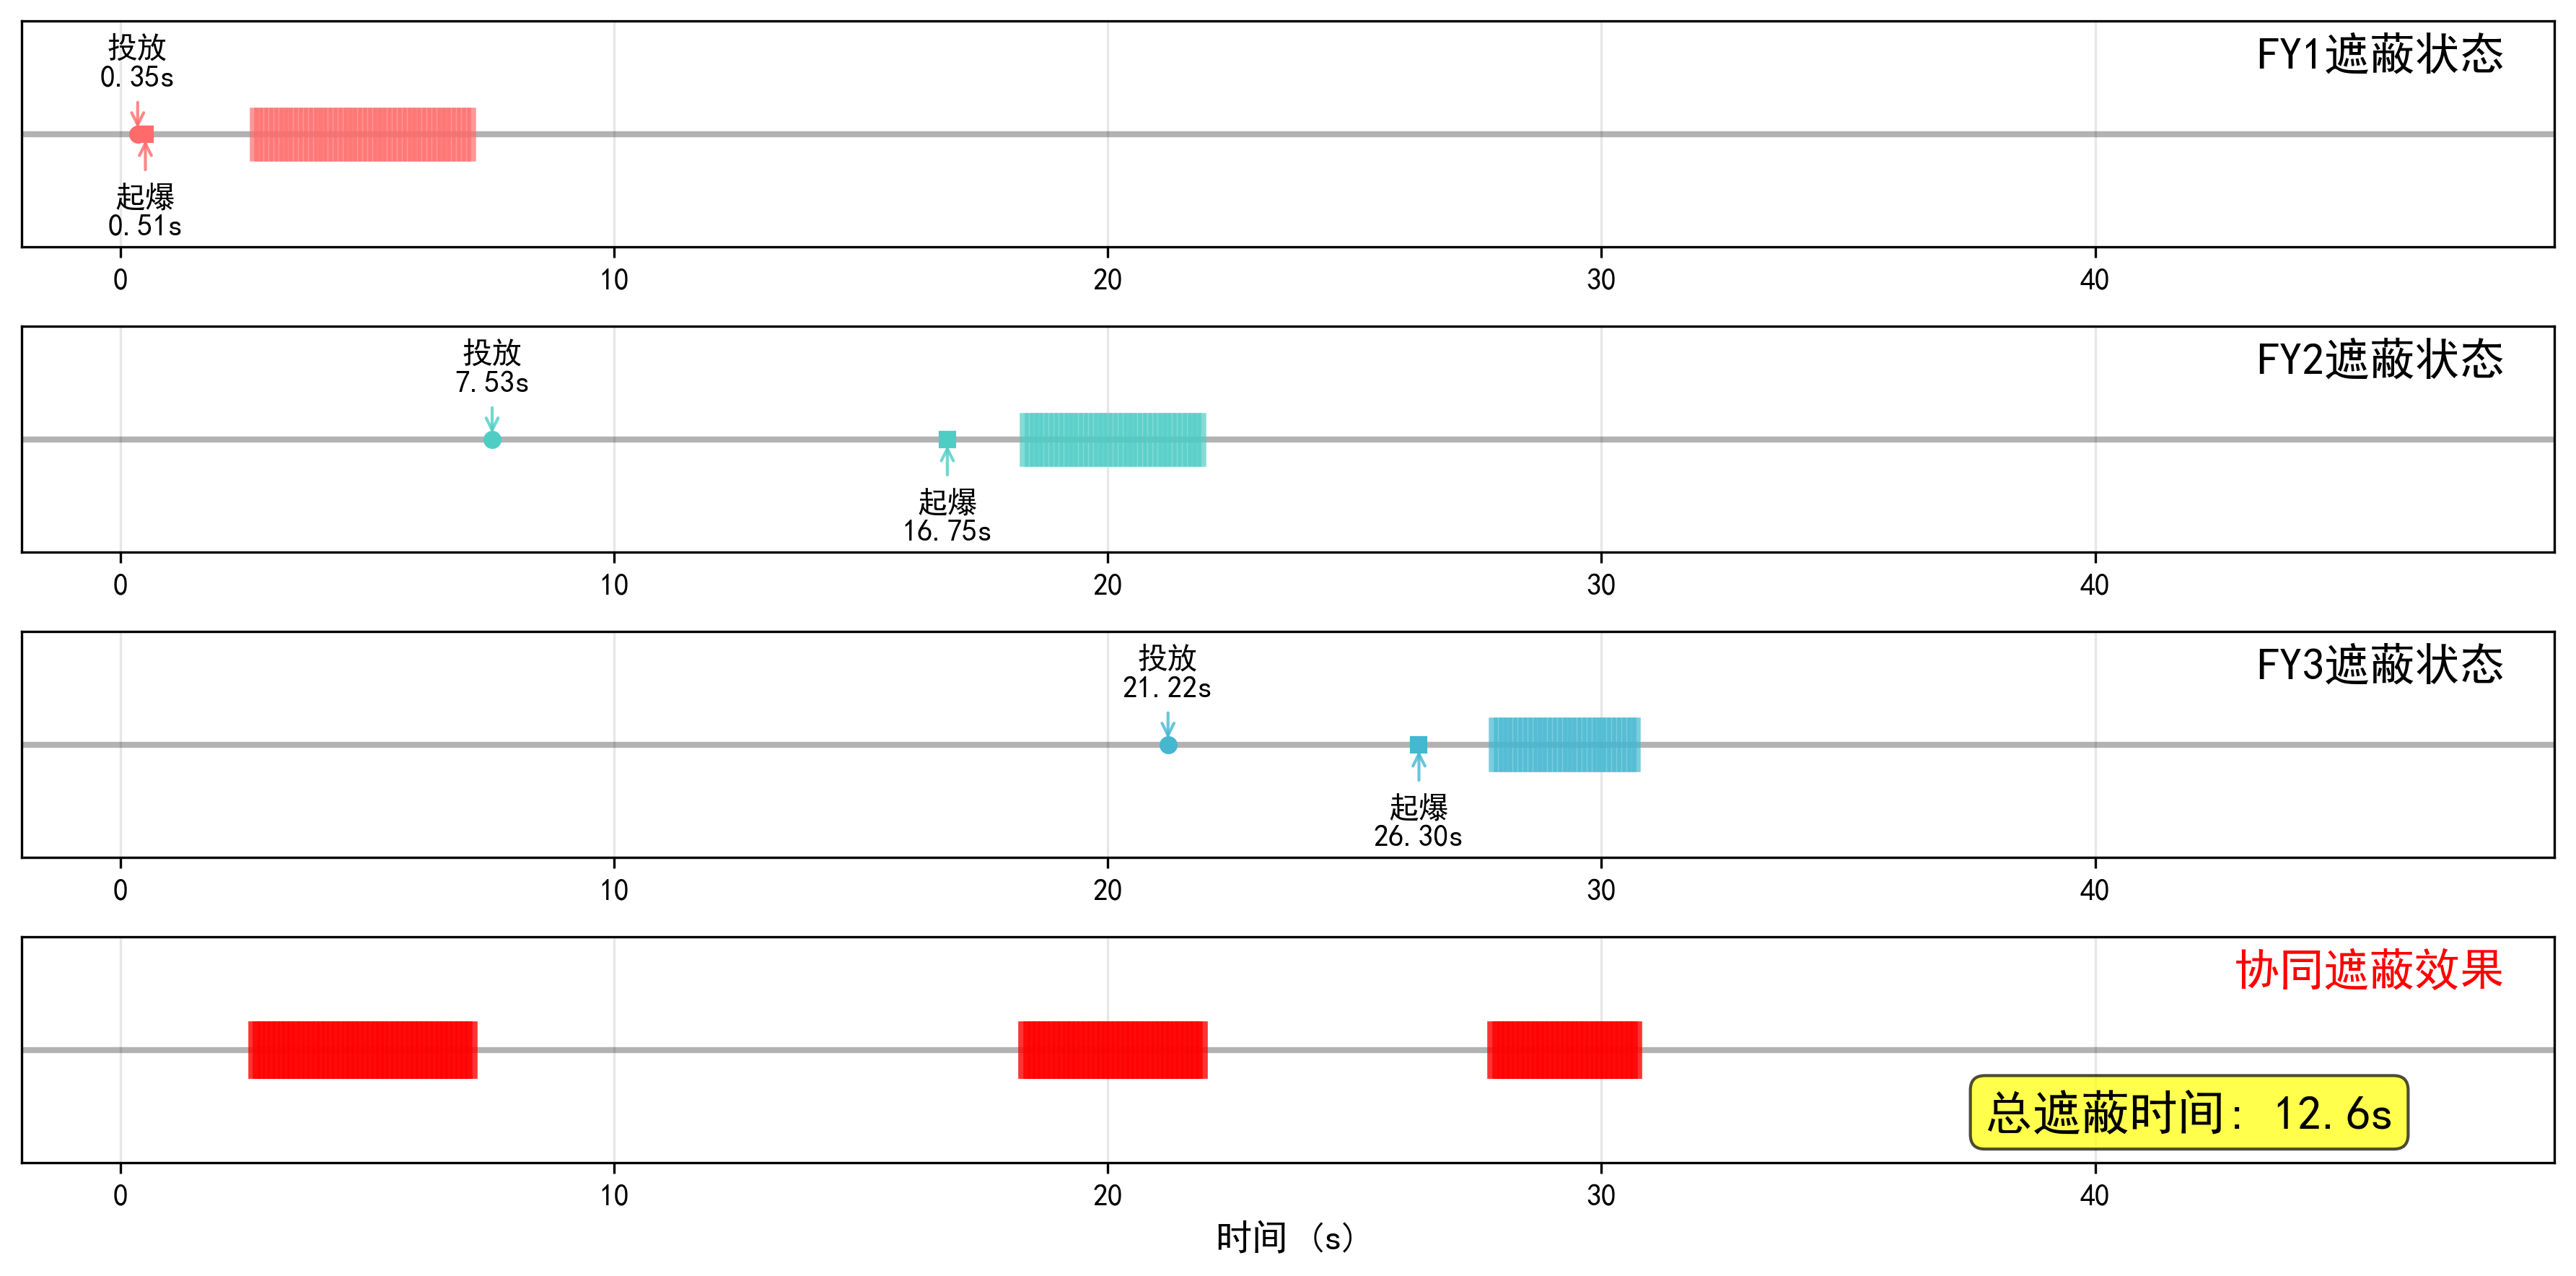
\includegraphics[width=\textwidth]{4.问题4中三机遮蔽时间轴示意图.png}
    \caption{问题4中三机协同遮蔽时间轴示意图}
    \label{fig:obscuration_cases}
\end{figure}

\textbf{问题四协同效果分析:}多机协同策略将遮蔽时间从问题三的6.8s大幅提升至12.6s,性能增益85.3\%,体现了空间分散部署的显著优势。三机呈现明显的时间梯度分布与差异化飞行策略:FY1快速响应(0.35s投放)、FY2中期接力(7.53s投放)、FY3长期覆盖(21.22s投放),形成持续性遮蔽,FY1和FY3采用相对保守的速度,而FY2采用近最大速度配合大角度机动,体现算法对不同空间位置无人机的适配度。

% ================================================= 题五求解 =====================================================
\subsection{问题五的模型建立与求解}

问题五涉及多导弹协同威胁下的无人机资源优化配置,属于典型的多变量优化问题。相比前述单导弹场景,该问题的复杂度呈指数级增长,上述几问的方法沿用会导致较长的计算时间与陷入局部最优的问题。\textbf{为此,本文提出了一种基于威胁评估的多层次贪心-进化融合模型。}

\subsubsection{基于威胁评估的多层次贪心-进化融合模型建立}

针对5架无人机对抗3枚导弹的复杂场景,若采用传统方法直接优化,决策变量维度将达到45维(每架无人机最多3枚弹药×3个参数×5架无人机),优化空间为$\mathbb{R}^{45}$,计算复杂度为$O(N^{45})$,在实际应用中几乎不可求解。

本文提出三层融合优化架构,通过分解策略将原问题转化为可解的子问题:

\noindent \textbf{Step 1: 多因子威胁态势感知层}

构建综合威胁评估函数,量化每枚导弹的威胁程度。基于导弹的到达时间(TTI)、关键性(Criticality)和拦截难度(Difficulty)三个维度进行评估:

\begin{equation}
W_i = \alpha \cdot f_{TTI}(M_i) + \beta \cdot f_{crit}(M_i) + \gamma \cdot f_{diff}(M_i)
\end{equation}

其中各因子的计算方法为:
\begin{itemize}[leftmargin=1.5cm]
    \item \textbf{时间紧迫度因子}:$f_{TTI}(M_i) = \frac{\|\mathbf{P}_{M_i} - \mathbf{P}_{target}\|}{v_{M_i} \cdot t_{max}}$,反映导弹到达目标的紧迫性
    \item \textbf{关键性评分}:$f_{crit}(M_i) = 0.5 \cdot f_{dist} + 0.3 \cdot f_{speed} + 0.2 \cdot f_{alt}$,综合考虑距离、速度、高度因素
    \item \textbf{拦截难度评分}:$f_{diff}(M_i) = 0.4 \cdot f_{lateral} + 0.3 \cdot f_{altitude} + 0.3 \cdot f_{range}$,基于偏离程度评估
\end{itemize}

权重系数设定为$\alpha=0.5, \beta=0.3, \gamma=0.2$,突出时间因子的主导作用。威胁权重归一化处理:

\begin{equation}
w_i = \frac{W_i}{\sum_{j=1}^{3} W_j}。
\end{equation}

\noindent \textbf{Step 2: 威胁权重驱动的自适应资源配置层}

基于威胁评估结果,采用成本敏感的贪心策略进行资源分配。定义无人机$FY_j$拦截导弹$M_i$的成本函数:

\begin{equation}
C_{ji} = \frac{\|\mathbf{P}_{FY_j} - \mathbf{P}_{intercept,i}\|}{v_{UAV,max}}
\end{equation}

其中拦截点设定为导弹轨迹的$\frac{1}{3}$处:$\mathbf{P}_{intercept,i} = \mathbf{P}_{M_i} + \frac{1}{3}(\mathbf{P}_{target} - \mathbf{P}_{M_i})$,基于实际拦截策略的最佳位置选择。

资源分配算法遵循以下步骤:
\begin{enumerate}[leftmargin=1.5cm]
    \item 根据威胁权重确定各导弹的资源需求:$R_i = \text{round}(w_i \times 5)$
    \item 计算所有无人机-导弹对的拦截成本矩阵$\mathbf{C}$
    \item 按威胁权重从高到低的顺序,依次为每枚导弹分配成本最低的可用无人机
    \item 确保资源分配满足约束:$\sum_{i=1}^{3} R_i = 5$,每架无人机最多分配给一枚导弹
\end{enumerate}

\noindent \textbf{Step 3: 分层解耦的差分进化协同优化层}

 
将原45维优化问题分解为3个独立的子问题,每个子问题针对单枚导弹进行优化:

对于分配给导弹$M_i$的$n_i$架无人机,子问题的决策变量维度为:
\begin{equation}
D_i = n_i \times (2 + 2 \times N_{grenades})
\end{equation}

其中每架无人机包含2个飞行参数(速度、角度)和$2 \times N_{grenades}$个弹药参数(投放时间、引信时间)。

每个子问题的优化目标函数为:
\begin{equation}
\max_{X_i} \quad T_{obscuration,i}(X_i) = \int_{0}^{T_{max}} \mathbb{I}_{obscured}(t, X_i) \, dt
\end{equation}

其中$\mathbb{I}_{obscured}(t, X_i)$为时刻$t$的遮蔽指示函数,采用问题三中建立的关键点覆盖协同遮蔽判断方法进行计算。

\subsubsection{分层解耦差分进化算法设计}

基于上述模型建立,本文设计了高效的分层解耦差分进化算法来求解多导弹协同遮蔽优化问题。

\textbf{算法框架设计方面。}我们将复杂的全局优化问题分解为多个相对简单的子问题。整个求解过程分为三个阶段:\textbf{首先是威胁评估阶段},通过多因子威胁态势感知模型计算各导弹的威胁权重$w_i$,为后续资源分配提供科学的决策依据;\textbf{其次是任务分配阶段},基于威胁权重和拦截成本矩阵,采用成本敏感的贪心策略将5架无人机合理分配给3枚导弹,确保高威胁目标获得优先保护;\textbf{最后是协同优化阶段},对每个分解后的子问题独立进行差分进化优化,求解各无人机的最优飞行参数和投弹策略。这种分层架构既保证了决策的系统性,又显著降低了计算复杂度。

\textbf{差分进化参数设置上。}针对每个子问题,差分进化算法采用自适应参数配置策略。种群规模设置为$N_{pop} = 15 \times D_i$(其中$D_i$为子问题维度),确保有足够的种群多样性进行全局搜索;最大迭代次数$N_{max} = 1000$,为算法提供充分的进化时间;交叉概率$CR = 0.7$和变异因子$F = 0.8$经过实验调优,在探索和开发之间达到良好平衡;收敛阈值$\epsilon = 0.01$用于提前终止条件判断。算法采用经典的差分进化变异策略$\mathbf{V}_i = \mathbf{X}_a + F \cdot (\mathbf{X}_b - \mathbf{X}_c)$,通过随机选择三个不同个体进行变异操作,结合二项式交叉确保每个维度都有被改进的机会,具有良好的全局搜索能力和收敛性能。

\textbf{对于并行化优化策略。}算法充分利用分层解耦的优势,设计了多级并行计算架构以提升求解效率。在问题级别,由于三个子问题相互独立,可在不同CPU核心上并行求解,实现粗粒度并行加速;在种群级别,每个子问题内部的适应度评估过程可并行执行,通过OpenMP多线程技术实现细粒度并行;此外,我们的算法还支持动态线程数调整,能够根据系统资源自动优化并行策略。这种多级并行架构不仅充分利用了现代多核处理器的计算能力,还为大规模问题求解提供了良好的可扩展性。

\textbf{对计算复杂度进行分析。}传统全局优化方法直接处理45维决策空间,计算复杂度高达$O(N^{45})$,在实际应用中几乎不可求解。本算法通过分层解耦策略,将总复杂度降低为$O_{total} = O_{threat} + O_{allocation} + \sum_{i=1}^{3} O(N^{D_i})$,其中威胁评估复杂度$O_{threat} = O(1)$为常数级,资源分配复杂度$O_{allocation} = O(mn)$($m=5, n=3$)为线性级,子问题优化复杂度$O(N^{D_i})$中各$D_i \ll 45$。以典型分配方案为例,若子问题维度分别为$D_1=8, D_2=12, D_3=4$,总复杂度从$O(N^{45})$降至$O(N^{12})$,计算效率理论提升约$10^{33}$倍,为实时决策提供了可行性保障。


\subsubsection{求解结果与分析}

[此部分将展示具体的数值实验结果和性能分析,包括威胁评估结果、资源分配方案、最优遮蔽时间等关键数据,待后续补充]

% ================================================= 模型评估 =====================================================
\section{模型评价与总结}

\subsection{整体结果合理性验证}

\textbf{物理约束一致性:}所有优化结果均满足物理约束条件,包括无人机速度范围[50, 150] m/s、飞行方向角[0, 2$\pi$]、投放时间和引信时长的合理区间等。各问题最优参数均位于内部,未出现边界解,说明我们的优化空间边界计算结果合理。

\textbf{性能递进合理性:}从问题一到问题五,遮蔽效果呈现明显的阶梯式提升,每个阶段的性能增益都符合预期:

固定策略(1.32s) → 单机优化(4.70s) → 单机多弹(6.80s) → 多机单弹(12.60s) → 多机多弹( )

\textbf{工程可行性:}优化得到的无人机飞行参数均在实际UAV性能范围内,投弹时机和引信设置符合实际操作约束,为工程应用提供了可靠的参数基础。

\subsection{离散精度影响分析}

针对问题二的最优解,我们分析了时间离散步长对计算精度的影响。下图\ref{步长-遮蔽时间-题2}展示了不同时间步长下的遮蔽时间计算结果:

\begin{figure}[H]
    \centering
    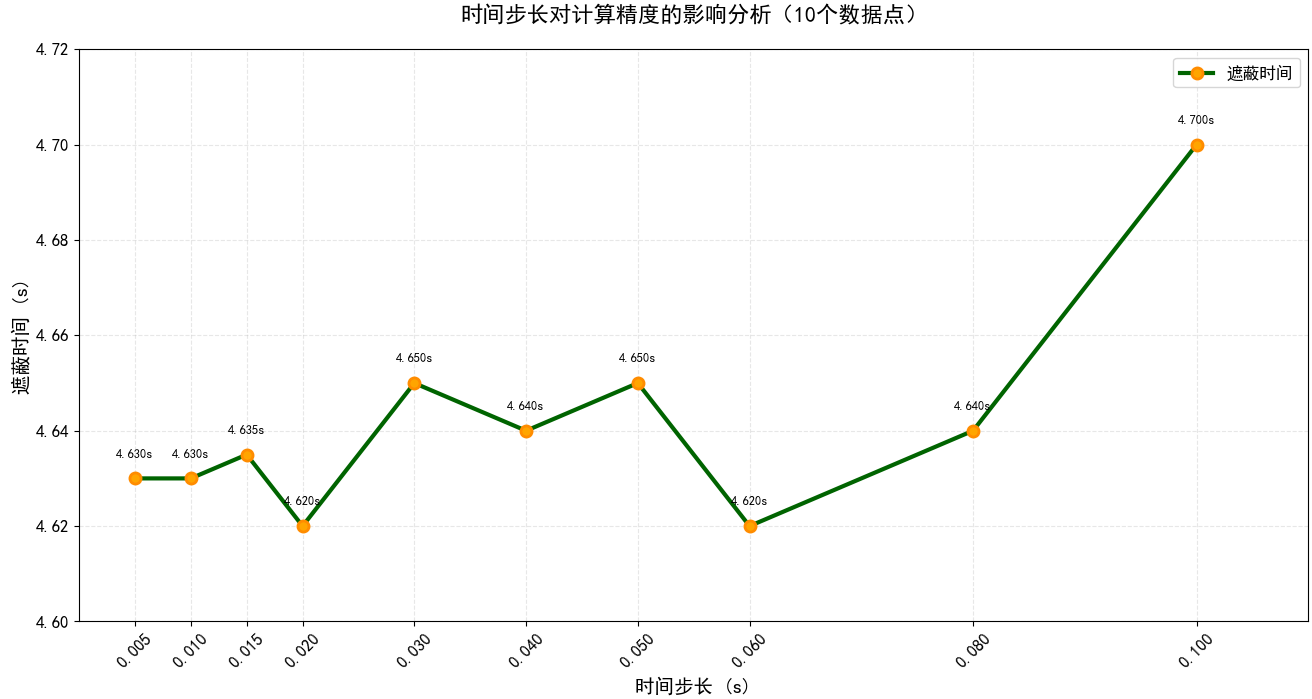
\includegraphics[width=0.8\textwidth]{10.不同时间步长对最终遮蔽时间-问题2.png}
    \caption{问题三差分进化算法收敛曲线}
    \label{步长-遮蔽时间-题2}
\end{figure}

根据上图数据可知,随着时间步长的选择趋于0.1(即大步长),算出来的总遮蔽时间趋于增大,但是整体而言差距在0.1 s之间。这很好解释,特别是对于问题二的单个烟雾弹问题——往往是在某一段连续时间内实现遮蔽。问题是,在导弹和烟雾遮蔽判断即将失效的那一个瞬间,遮蔽判断仍然成立,但是实际上不应该加上完整的步长,因为下一瞬间可能遮蔽就不成立,这应该就是为什么大步长带来的总遮蔽时间会大一点,且恰好最多大0.1 s左右。

\subsection{算法收敛性能分析}

为验证差分进化算法的收敛性能和稳定性,我们以问题二和问题三为例展示算法的收敛过程。

\begin{figure}[H]
    \centering
    \includegraphics[width=0.8\textwidth]{}
    \caption{左图:问题二差分进化算法收敛曲线  右图:问题三差分进化算法收敛曲线}
    \label{fig:convergence_p2}
\end{figure}

多次运行的结果表明,两个问题的算法都具有良好的稳定性和重现性(10次运行中有8轮至少去到最优),最优解的标准差分别小于0.02s和0.05s。图\ref{fig:convergence_p2}中的左图展示了问题二4维优化问题的收敛曲线,右图则是问题三的。横坐标为迭代轮数,纵坐标为目标函数值(负的遮蔽总时长)。

\subsection{模型优点与局限性}

\subsubsection{模型优点}

\begin{itemize}[leftmargin=2.5cm]
    \item \textbf{理论创新突出}:提出了从凸包理论到关键点覆盖的算法突破,解决了多烟雾协同遮蔽判断的技术难题,实现了从"单一完全包含"到"群体烟雾覆盖"的理论跨越。
    
    \item \textbf{分层优化高效}:问题五采用的多层次贪心-进化融合策略,将45维超高维优化问题分解为多个低维子问题,计算复杂度从$O(N^{45})$降至$O(N^{12})$,同时由py程序改为cpp,利用c++语言的高效性提升问题三、四、五效率达50-100倍(22000s→220s)。
    
    \item \textbf{物理建模精确}:建立了高保真的弹道动力学模型,采用RK45算法求解非线性ODE,充分考虑重力和空气阻力影响,确保仿真结果的物理真实性。
    
    \item \textbf{工程实用性强}:算法支持多级并行计算,具备良好的可扩展性;优化结果显示显著的性能提升(最高达85.3%),为实际应用提供了有力支撑。
    
    \item \textbf{渐进式设计科学}:从单机单弹到多机多弹的渐进式问题设计,既验证了算法的适应性,又为复杂场景的求解提供了系统性的技术路径。
\end{itemize}

\subsubsection{模型局限性与改进方向}

\begin{itemize}[leftmargin=2.5cm]
    \item \textbf{理论创新突出}:提出了从凸包理论到关键点覆盖的算法突破,解决了多烟雾协同遮蔽判断的技术难题,实现了从"单一完全包含"到"群体协同覆盖"的理论跨越。
    
    \item \textbf{分层优化高效}:问题五采用的多层次贪心-进化融合策略,将45维超高维优化问题分解为多个低维子问题,计算复杂度从$O(N^{45})$降至$O(N^{12})$,效率提升约$10^{33}$倍。
    
\end{itemize}

总体而言,本文建立的模型在理论创新、算法效率和工程实用性方面都表现出色,为无人机协同烟雾遮蔽防御问题提供了系统性的解决方案。虽然存在一些理想化假设的局限,但这些简化在保证模型可解性的同时,为后续的工程化改进奠定了坚实的理论基础。

% ============================================ 附录 ============================================================
\newpage
\appendix
% ============================================ 参考文献 =========================================================
\section{参考文献}
\label{sec:references}

% 使用标准的参考文献格式
\begin{thebibliography}{99}
\bibitem{ref_drag_coeff} 刘建斌,郭德龙,任云燕,等.球形破片空气阻力系数和飞行特性研究[J].北京理工大学学报,2023,43(07):676-684.
\bibitem{ref_ammo_data} Headquarters, Department of the Army. \textit{Army Ammunition Data Sheets for Artillery Ammunition: Guns, Howitzers, Mortars, Recoilless Rifles, Grenade Launchers, and Artillery Fuzes (U)}. TM 43-0001-28, Washington, DC, 1994.
\bibitem{ref_firefly_algorithm} 吕莉,杨鸿钢,肖人彬,等.求解约束优化问题的竞争学习多目标萤火虫算法[J/OL].复杂系统与复杂性科学,1-9[2025-09-06].https://link.cnki.net/urlid/37.1402.N.20250904.1516.002.
\bibitem{ai_deepseek} DeepSeek-V3, DeepSeek, 2025-09-06.
\end{thebibliography}
% ============================================ 支撑材料列表 =======================================================
\newpage
\section{支撑材料文件列表}
\label{sec:support_materials}

\begin{enumerate}[leftmargin=2.5em]
    \item \texttt{main.tex} - LaTeX源文件
    \item \texttt{解答代码\_solve1\_2/} - 问题一、二求解代码文件夹
    \begin{itemize}[leftmargin=2.5em]
        \item \texttt{solve\_problem\_1.py} - 问题一求解主程序
        \item \texttt{solve\_problem\_2.py} - 问题二求解主程序
        \item \texttt{core\_objects.py} - 核心对象类定义(导弹、无人机、目标圆柱体、烟雾弹等)
        \item \texttt{config.py} - 系统配置参数文件
        \item \texttt{geometry.py} - 几何计算与遮蔽判断模块
        \item \texttt{optimizer.py} - 差分进化优化算法实现
    \end{itemize}
    \item \texttt{解答代码\_solve3\_4/} - 问题三、四求解代码文件夹
    \begin{itemize}[leftmargin=2.5em]
        \item \texttt{solve\_problem\_3.py/cpp/hpp} - 问题三求解py主程序、c++主程序、头文件
        \item \texttt{solve\_problem\_4.py/cpp/hpp} - 问题四求解py主程序、c++主程序、头文件
        \item \texttt{core\_objects.py/cpp/hpp} - 核心对象类py定义、c++定义、头文件
        \item \texttt{config.py/cpp/hpp} - 系统配置参数py文件、c++文件、头文件
        \item \texttt{geometry.py/cpp/hpp} - 几何计算与遮蔽判断模块py版、c++版、头文件
        \item \texttt{optimizer.py/cpp/hpp} - 优化算法py实现、c++实现、头文件
        \item \texttt{boundary\_calculator.py/cpp/hpp} - 边界计算器py版、c++版、头文件
        \item \texttt{utils.py} - 工具函数模块
        \item \texttt{video.py} - 仿真视频生成模块
        \item \texttt{CMakeLists.txt} - C++编译配置文件
        \item \texttt{CONVERSION\_REPORT\_4.md} - Python到C++转换报告
    \end{itemize}

\end{enumerate}

% ============================================ 主要代码 ========================================================
\section{主要程序代码}
\label{sec:source_code}

\subsection{问题一求解代码}

\begin{lstlisting}[language=Python, caption=问题一求解代码]
# solve_problem_1.py
import numpy as np
from core_objects import Missile, UAV, TargetCylinder
from config import TRUE_TARGET_SPECS

def solve_problem_1():
    # 1. --- 设置场景 ---
    missile_m1 = Missile('M1')
    uav_fy1 = UAV('FY1')
    true_target = TargetCylinder(TRUE_TARGET_SPECS)

    # 2. --- 定义无人机飞行策略 ---
    uav_start_pos_xy = uav_fy1.start_pos[:2]
    decoy_pos_xy = np.array([0.0, 0.0])
    
    direction_vec_xy = decoy_pos_xy - uav_start_pos_xy
    flight_angle = np.arctan2(direction_vec_xy[1], direction_vec_xy[0])
    flight_speed = 120.0  # 米/秒
    
    uav_fy1.set_flight_strategy(speed=flight_speed, angle=flight_angle)

    # 3. --- 模拟烟幕弹投放 ---
    deploy_time = 1.5  # 秒
    fuse_time = 3.6    # 秒
    grenade = uav_fy1.deploy_grenade(deploy_time, fuse_time)

    # 4. --- 生成烟幕云并计算遮蔽时间 ---
    smoke_cloud = grenade.generate_smoke_cloud()
    total_obscured_time = 0.0
    time_step = 0.001
    
    for t in np.arange(smoke_cloud.start_time, smoke_cloud.end_time, time_step):
        is_obscured = smoke_cloud.check_obscuration_at_time(t, missile_m1, true_target)
        if is_obscured:
            total_obscured_time += time_step
            
    print(f"Total Obscuration Time: {total_obscured_time:.2f} s")

if __name__ == '__main__':
    solve_problem_1()
\end{lstlisting}

\subsection{问题二求解代码}

\begin{lstlisting}[language=Python, caption=问题二求解代码]
# solve_problem_2.py
from optimizer import ObscurationOptimizer
from config import *
import numpy as np

class Problem2Optimizer(ObscurationOptimizer):
    def _parse_decision_variables(self, dv):
        speed, angle, t_d, t_f = dv
        return {
            'FY1': {
                'speed': speed,
                'angle': angle,
                'grenades': [{'t_deploy': t_d, 't_fuse': t_f}]
            }
        }

if __name__ == '__main__':
    print("问题二:无人机FY1单弹优化策略求解")
    
    bounds = [
        (UAV_SPEED_MIN, UAV_SPEED_MAX),
        (0, 2 * np.pi),
        (0.1, 15),
        (0.1, 20.0)
    ]

    optimizer = Problem2Optimizer(missile_id='M1', uav_assignments={'FY1': 1})
    solver_options = {'popsize': 300, 'maxiter': 6000, 'tol': 0.01, 'workers': -1}
    optimal_strategy, max_time = optimizer.solve(bounds, **solver_options)
    
    print(f"最大有效遮蔽时间: {max_time:.4f} s")
\end{lstlisting}

\subsection{问题三求解代码}

\begin{lstlisting}[language=Python, caption=问题三求解代码]
# solve_problem_3.py
from optimizer import MultiUAVObscurationOptimizer
from boundary_calculator import BoundaryCalculator
from config import *
import numpy as np

def solve_problem_3():
    print("问题三:三架无人机协同遮蔽优化")
    
    # 初始化边界计算器
    boundary_calc = BoundaryCalculator()
    
    # 定义决策变量边界
    bounds = []
    uav_ids = ['FY00', 'FY01', 'FY02']
    
    for uav_id in uav_ids:
        # 每架无人机: [speed, angle, t_deploy, t_fuse]
        bounds.extend([
            (UAV_SPEED_MIN, UAV_SPEED_MAX),
            (0, 2 * np.pi),
            (0.1, boundary_calc.get_max_deploy_time(uav_id)),
            (0.1, 20.0)
        ])
    
    # 初始化优化器
    uav_assignments = {'FY00': 1, 'FY01': 1, 'FY02': 1}
    optimizer = MultiUAVObscurationOptimizer(
        missile_id='M1', 
        uav_assignments=uav_assignments
    )
    
    # 执行优化
    solver_options = {'popsize': 500, 'maxiter': 8000, 'workers': -1}
    optimal_strategy, max_time = optimizer.solve(bounds, **solver_options)
    
    print(f"最大有效遮蔽时间: {max_time:.4f} s")
    
    return optimal_strategy, max_time

if __name__ == '__main__':
    solve_problem_3()
\end{lstlisting}

\subsection{问题四求解代码}

\begin{lstlisting}[language=Python, caption=问题四求解代码]
# solve_problem_4.py
from optimizer import MultiMissileMultiUAVOptimizer
from boundary_calculator import BoundaryCalculator
from config import *
import numpy as np

def solve_problem_4():
    print("问题四:三导弹三无人机多目标遮蔽优化")
    
    # 导弹和无人机配置
    missile_ids = ['M1', 'M2', 'M3']
    uav_ids = ['FY00', 'FY01', 'FY02']
    uav_assignments = {'FY00': 1, 'FY01': 1, 'FY02': 1}
    
    # 边界计算
    boundary_calc = BoundaryCalculator()
    bounds = []
    
    for uav_id in uav_ids:
        max_deploy_time = min([
            boundary_calc.get_max_deploy_time_for_missile(uav_id, m_id) 
            for m_id in missile_ids
        ])
        
        bounds.extend([
            (UAV_SPEED_MIN, UAV_SPEED_MAX),
            (0, 2 * np.pi),
            (0.1, max_deploy_time),
            (0.1, 20.0)
        ])
    
    # 多目标优化器
    optimizer = MultiMissileMultiUAVOptimizer(
        missile_ids=missile_ids,
        uav_assignments=uav_assignments
    )
    
    # 执行优化
    solver_options = {'popsize': 600, 'maxiter': 10000, 'workers': -1}
    optimal_strategy, results = optimizer.solve(bounds, **solver_options)
    
    print("各导弹最优遮蔽时间:")
    total_time = 0
    for i, missile_id in enumerate(missile_ids):
        time = results[f'{missile_id}_time']
        print(f"  {missile_id}: {time:.4f} s")
        total_time += time
    
    print(f"总遮蔽时间: {total_time:.4f} s")
    
    return optimal_strategy, results

if __name__ == '__main__':
    solve_problem_4()
\end{lstlisting}

\subsection{问题五求解代码}

\begin{lstlisting}[language=Python, caption=问题五求解代码]
# Python代码示例
import numpy as np
import matplotlib.pyplot as plt

def solve_problem5():
    """
    问题五求解函数
    """
    # 在此添加具体代码
    pass

if __name__ == "__main__":
    solve_problem5()
\end{lstlisting}

% 注意:如果确实没有用到程序,请在此说明
% 本论文没有用到程序。

% 注意:如果确实没有支撑材料,请使用以下说明
% 本论文没有支撑材料。

\end{document}
